\documentclass{article} % For LaTeX2e
\usepackage{iclr2026_conference,times}

\input{math_commands.tex}

\usepackage{hyperref}
\usepackage{url}
\usepackage{graphicx}
\usepackage{booktabs}
\usepackage{amsmath,amssymb,amsthm}
\usepackage{multirow}
\usepackage{subcaption}
\usepackage{algorithm}
\usepackage{algpseudocode}
\usepackage{float}
\usepackage{tikz}
\usetikzlibrary{arrows.meta,positioning,calc}

\newtheorem{theorem}{Theorem}
\newtheorem{proposition}{Proposition}
\newtheorem{corollary}{Corollary}
\newtheorem{definition}{Definition}

\newcommand{\bind}{\mathrm{bind}}
\newcommand{\cl}{\mathrm{cl}}
\newcommand{\VoI}{\mathrm{VoI}}
\newcommand{\feasible}{\mathrm{feasible}}
\newcommand{\Comp}{\mathrm{Comp}}
\newcommand{\bbot}{\bot}

\title{When the Evidence Cannot Decide:\\ Selective Right-Sizing of AI Deployments}

% Anonymous submission: do not set \iclrfinalcopy
\author{Anonymous authors}

\begin{document}

\maketitle

\begin{abstract}
Practitioners size AI deployments against public evaluation evidence, assuming the open problem is \emph{estimate quality}. We ask a prior question: given the evidence that exists, is the decision \emph{identified at all}? We formalize \emph{evidence-decidability} and measure it over 1{,}716 right-sizing queries from documented production deployments. The finding is a \textbf{certified floor}: under the most conservative modelling choices the framework admits, \textbf{41.0\%} of decisions are underdetermined by a measurable co-location gap alone---irreducible, because its source is which axes are measured, not how well, so no re-running of existing benchmarks shrinks it. The floor rises monotonically as assumptions are added: \textbf{56.9\%} under any bounded belief about the measurable axes, up to an \textbf{adversarial ceiling of 91.1\%} if every declared governance constraint is granted as binding. We flag the ceiling as exceeding our own evidence: the strongest binding anchor we can measure (a structured US-federal field) is \textbf{34.5\%}, and at that anchor the rate is 48.1\% under any bounded belief---well below the ceiling. The gap has teeth: the automated-tooling default---ranking on visible axes alone---violates the hidden quality constraint on \textbf{57.1\%} of decisions (CI [46.8, 67.6]); imputation does not repair it, and a calibrated-transfer interval recovers only a guaranteed minority, \emph{certifying} the rest require measurement. The selective procedure abstains, names the blocking measurement, and---closing the loop with real acquisition---reaches full coverage with zero violations.
\end{abstract}

\section{Introduction}
\label{sec:intro}

Every tool that helps a practitioner deploy a language model answers the same question: \emph{given this task and its constraints, what is the smallest configuration that suffices?} The community has invested enormously in sharpening the inputs: holistic benchmarks widen the metrics per model \citep{liang2022helm}, cost-aware agent evaluations add real dollars to accuracy \citep{kapoor2024agents,stroebl2025hal}, and routers drive cost down under an observed objective \citep{chen2023frugalgpt,hu2024routerbench,ong2024routellm}. All share a tacit premise: the frontier is \emph{estimate quality}, so a sharper belief about each model property yields a better decision.

This paper flips that premise into a measurable question. Before asking how precise the evidence is, we ask whether the deployment decision is \emph{identified at all} by the evidence that exists. We call a decision \emph{evidence-decidable} when the evidence pins down the optimum, and \emph{underdetermined} when two states of the world, both consistent with everything measured, disagree about which configuration to deploy. Underdetermination is not imprecision: no amount of re-running the present benchmarks shrinks it, because its source is which properties are measured, not how well.

\begin{figure}[t]
\centering
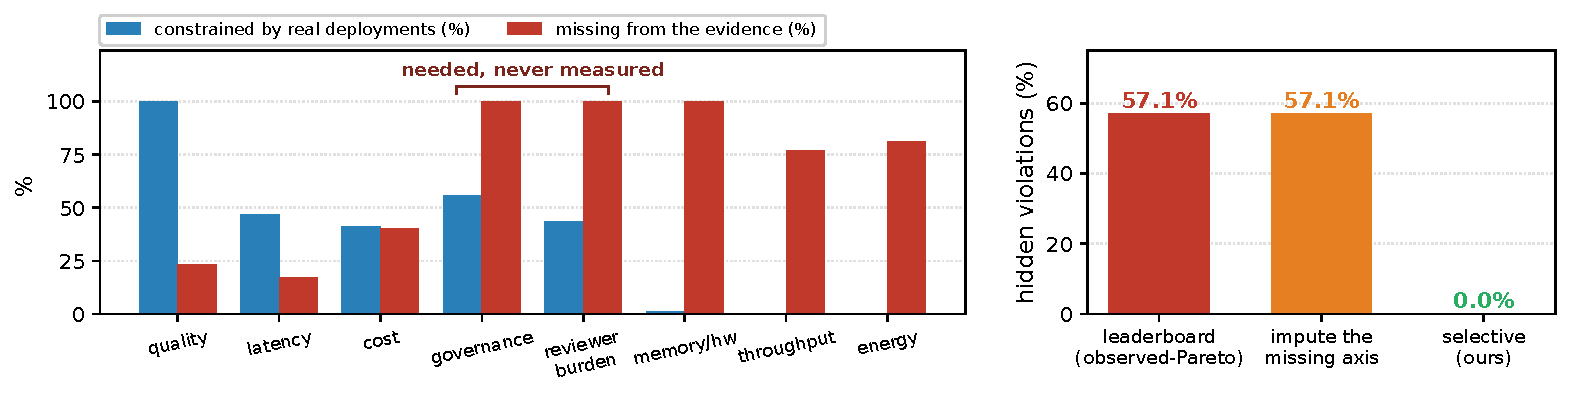
\includegraphics[width=0.56\linewidth]{figures/fig_teaser.pdf}
\caption{\textbf{The evidence and the decisions it must support are misaligned, and deciding anyway silently fails.}
\textbf{Left:} per deployment axis, the fraction of 1{,}716 documented deployments declaring it a constraint (blue) versus the fraction of configurations for which public evidence is silent (red); governance and reviewer burden are constraints in roughly half of deployments and unmeasured for \emph{every} configuration.
\textbf{Right:} on 476 ground-truth decisions with the binding \emph{quality} axis hidden, ranking on the visible axes silently violates the hidden quality constraint on 57.1\% of decisions, while the selective procedure abstains and names the resolving measurement (zero violations, 95\% CI [46.8, 67.6]). The 57.1\% is on the measurable quality axis, not on governance.}
\label{fig:teaser}
\end{figure}

Making this question empirical requires two artifacts that prior evaluation work does not provide. The first is an \emph{evidential substrate}: a relational store of provenance-tracked observations from public evaluation sources, in which missingness is derived from the absence of evidence and never imputed. The second is a \emph{grounded query distribution}: rather than inventing queries, we derive one right-sizing query from each of 1{,}716 documented production LLM deployments, so the result is a property of real deployment demand rather than of a grid we chose (Section~\ref{sec:substrate}).

The measurement makes the mismatch quantitative (Section~\ref{sec:map}), and Figure~\ref{fig:teaser} (left) shows it in one view. Our finding is a \textbf{certified floor of 41.0\%}, established under the most conservative modelling choices the framework admits and irreducible by better estimates. It rises monotonically as assumptions are added---\textbf{56.9\%} under any bounded belief about the measurable axes, to an \textbf{adversarial ceiling of 91.1\%} granting that declared constraints bind. We lead with the floor because it alone is robust to every modelling choice; the ceiling is a labelled upper bound that, as we show (Section~\ref{sec:map}), exceeds what our own binding anchors support (at most 34.5\%). The picture survives every confidence-filter, single-tag deletion ($\ge 83.2\%$), adversarial re-weighting ($\ge 95.7\%$), corpus scaling, and three independent-corpus replications.

A measurement of underdetermination would be a curiosity if deciding anyway were harmless. Our second result shows it is not (Section~\ref{sec:validation}). On 28 corpus slices where ground truth for a \emph{binding axis} (a constraint active at the optimum, whose relaxation would change the cheapest-sufficient configuration) exists, we hide that axis, let each rule commit from what remains, and score against the hidden truth. The automated-tooling default---rank on visible axes, pick the cheapest acceptable configuration---silently \emph{violates the hidden constraint} on 57.1\% of decisions (slice-clustered 95\% CI [46.8, 67.6]); median imputation commits the identical violations, and a \emph{learned} imputer with genuine cross-context signal halves but does not repair them. Our end-to-end procedure---abstain, measure the named axes, then commit---reaches the same full coverage with \emph{zero} violations. This harm is necessarily scored on \emph{measurable} axes; on the blind-spot axes the validation is impossible, itself the finding.

Refusal alone would be cheap, but the procedure's abstention is \emph{informative}: it returns the blocking axes and a value-of-information (VoI) ranking of which measurement resolves the decision per unit cost, grounded in a regret-floor identity $\VoI=\Delta=\delta\lambda/(\delta+\lambda)$ that our implementation matches to machine precision (Section~\ref{sec:theory}). When two axes genuinely block, neither sufficient alone, the ranked plan resolves every decision in 2.0 measurements against 6.0 for unplanned probing, and a calibrated margin keeps feasibility risk below $\alpha=5\%$ at 89\% coverage (Sections~\ref{sec:validation},~\ref{sec:resolve}). This is the delta from selective prediction, which abstains on low \emph{model} confidence \citep{chow1970optimum,elyaniv2010foundations}: \textbf{our trigger is non-identifiability from missing evidence, and the abstention is informative}, returning the measurement that resolves the decision with a proved link to the regret floor.

\textbf{Contributions.}
\begin{enumerate}
\item \textbf{A reframing with an operational measure}: right-sizing as an identifiability question, with a verdict (decidable / underdetermined / infeasible) computable from any evidence corpus, conservative so that every reported underdetermination rate is a lower bound (Section~\ref{sec:setup}). In practice the verdict is two-valued; the infeasible label is empirically empty (0/1{,}716).
\item \textbf{To our knowledge, the first decidability map over realistically distributed deployment queries}, reported as a labelled assumption envelope: a \textbf{certified floor of 41.0\%} robust to all modelling choices (the finding), a belief-robust \textbf{56.9\%}, and an \textbf{adversarial ceiling of 91.1\%} that we explicitly flag as exceeding our measured binding anchors (at most 34.5\%)---so the floor, not the ceiling, carries the claim. The blind spot is \textbf{82.5\%} co-location failures on measurable axes and \textbf{17.5\%} structural absences, of which only \textbf{20.5\%} are \emph{purely} measurable; robust to confidence policy, taxonomy, query distribution, corpus scale, and \emph{three} independent-corpus replications (Section~\ref{sec:map}).
\item \textbf{Evidence that deciding anyway fails, and what a guarantee can and cannot recover}: imputation is a no-op (57.1\% violation rate unchanged); a learned imputer halves it (30.6\%); Bayesian/CC rules escape only by $70{\times}$--$127{\times}$ over-provisioning. A \emph{calibrated-transfer interval} fed to the same verdict recovers \textbf{24.9\%} of co-location decisions at \emph{zero} violations with $P(\text{infeasible}\mid\text{commit})\le\alpha$, certifying the rest require measurement (Appendix~\ref{app:transfer}). The selective procedure is the only method achieving \emph{both} zero violations and full coverage ($n{=}476$, CI [46.8, 67.6]; Section~\ref{sec:validation}).
\item \textbf{The resolution trichotomy and a selective procedure that acts on it}: every underdetermined decision is cured by transfer, resolved by measurement, or structurally unmeasured (Section~\ref{sec:resolve}). The procedure commits, abstains-and-names-the-measurement, or reports infeasible; its live acquisition loop resolves two genuine blockers in 2.0 real measurements versus 6.0 for unplanned probing, with zero violations and minimum-sufficient commitments, and the named measurement's VoI equals the minimax committed regret (Theorem~\ref{thm:general}).
\end{enumerate}
We contribute both halves. The first is a \emph{diagnosis} of the evaluation ecosystem: public benchmarks measure model properties, while deployments are gated by configuration- and jurisdiction-level properties no source publishes. The second is two \emph{guaranteed methods} that act on the diagnosis. We organize them by a partition we name the \emph{resolution trichotomy}: an underdetermined decision is cured by transfer, resolved by measurement, or structurally unmeasured, and the methods diagnose the gap, cure its co-location part with calibrated transfer, close the loop on the rest with real acquisition, and name the governance part no evidence can yet decide (Section~\ref{sec:resolve}).

\section{Related Work}
\label{sec:related}

\textbf{Better estimates, same identifiability assumption.}
HELM \citep{liang2022helm} broadens the metrics reported per model and is precisely the kind of evidence our substrate ingests, but it produces a richer estimate, not a statement of when that estimate suffices to identify a deployment choice. \citet{kapoor2024agents} show that accuracy-only agent evaluation misleads and argue for joint accuracy--cost Pareto analysis; the Holistic Agent Leaderboard \citep{stroebl2025hal} makes the estimate far more reliable with 21{,}730 instrumented rollouts. Our result is one step before theirs: even a joint accuracy--cost rule still answers decisions it cannot identify, because real deployments also bind latency, energy, governance, and reviewer burden---axes a Pareto front over reported metrics never sees. Frugal routers \citep{chen2023frugalgpt,hu2024routerbench,ong2024routellm,chen2025llmselector} optimize selection \emph{under an observed objective}, but in our setting the objective or a binding constraint is frequently unobserved (cost evidence is absent for 75.1\% of the derived queries), so there is nothing to frugally minimize until the axis is measured. The lines are complementary: on the decidable slice, frugal optimization is exactly what should run, as it is for runtime planners and cascade serving systems \citep{circinus2025,cascadia2025} that likewise treat system properties as known.

\textbf{Selective prediction and conformal guarantees.}
Abstention under uncertainty goes back to \citet{chow1970optimum} and was formalized by \citet{elyaniv2010foundations,geifman2017selective}, with distribution-free risk control via conformal methods \citep{angelopoulos2023conformal}. Trust-or-Escalate \citep{jung2025trust} applies the selective shape to LLM judging with a coverage-at-agreement guarantee. We adapt the selective-commit skeleton with three formal differences: the committed object is a multi-constraint feasibility-and-minimality decision, not a binary label; the trigger is non-identifiability from missing evidence, not low model confidence; and the abstention is informative, returning the measurement that resolves the decision with a proved link to the regret floor. \citet{dorner2025limits} prove that a judge no better than the evaluated model cannot substitute for more labels; our limit result is structurally parallel in a different currency---evidence on the wrong axes cannot substitute for measuring the binding one, no matter how abundant.

\textbf{Missing data and partial identification.}
Our never-impute stance follows the partial-identification tradition \citep{manski2003partial}: when data cannot identify a quantity, report the identified set rather than a point. The missingness we measure is non-ignorable in the strongest classical sense \citep{rubin1976inference,little2019statistical}---entire axes are absent because nobody measures them---which is why imputation fails empirically in Section~\ref{sec:validation}. Value-of-information is classical \citep{howard1966voi}; our contribution is the identity tying an implementable VoI to a regret floor indexed by which axes carry evidence.

\section{Problem Setup: Right-Sizing under Partial Evidence}
\label{sec:setup}

\subsection{Queries, configurations, axes}

A \textbf{configuration} $x \in \mathcal{X}$ is a fully specified deployable assembly: model, context length, retrieval, decoding, orchestration. A \textbf{task archetype} $\tau$ names a workload (general QA, function calling, inference serving), and $\mathcal{X}(\tau)$ is the admissible set. Right-sizing is judged on eight \textbf{axes} $A = \{$quality, latency, throughput, cost, energy, memory/hw, governance, reviewer burden$\}$: the first five are familiar benchmark quantities; \emph{governance} is regulatory admissibility (a compliance regime the deployment must satisfy), \emph{reviewer burden} is the human-review budget it consumes, and \emph{memory/hw} is the on-device envelope. Each axis has a true value $\theta_a(x)$, never observed directly. A \textbf{query} $q = (\tau, c)$ carries a constraint bundle $c$ of (axis, relation, threshold) triples, e.g.\ quality $\ge 0.8$ and latency $\le$ 2s. The oracle target is the \textbf{cheapest sufficient configuration}
$x^*(q) = \arg\min_{x \in \mathcal{X}(\tau):\,\feasible(x,c)} \mathrm{cost}(x)$,
a textbook constrained optimum on purpose: everything novel happens when $\theta$ is replaced by partial evidence about $\theta$. We write $\bind(q) \subseteq A$ for the axes whose constraints are \emph{active} at the optimum---those whose relaxation would change $x^*(q)$.

\subsection{Observations, confidence, and derived missingness}

The evidence base $E$ is a set of \textbf{observations}: tuples $\langle \text{value},\ \text{confidence} \in \{H,M,L\},\ \text{source},\ \text{context} \rangle$ for a cell $(x,a)$, where $H$ is direct measurement, $M$ leaderboard or paper-reported, $L$ vendor claims; context records dataset, split, hardware, and date so commensurability is checkable. A solver chooses a confidence policy $\kappa$ (default $\{H,M\}$) and an aggregation $\varphi$, and the \textbf{belief} about a cell is derived at query time from the $\kappa$-filtered observations. In this paper $\varphi$ maps those observations to an \emph{interval}: the min--max of commensurable observed values, collapsing to a point when they agree. A belief \emph{straddles} a threshold when its interval contains it. The central definition is that \emph{missingness is derived, not stored}:
\begin{equation}
B_E(x,a) = \bbot \iff \text{the $\kappa$-filtered observation set for $(x,a)$ is empty.}
\end{equation}
A missing cell stays missing: we never fill $\bbot$ with a prior, a median, or a model---Section~\ref{sec:validation} shows imputation reproduces exactly the failures it is meant to avoid.

\subsection{Three verdicts, and decidability via possible worlds}
\label{sec:decidability}

Fix a query and a policy. Each candidate is certified per constraint against its belief: \emph{satisfied}, \emph{violated}, or \emph{undetermined} (the constraint's axis is $\bbot$ or the belief straddles the threshold). Let $\Comp(E)$ be the set of \textbf{completions} of $E$: a completion assigns each $\bbot$ cell any value in its axis domain and each straddling cell any value in its observed interval---the possible worlds the evidence cannot rule out.

\begin{definition}[Evidence-decidability]
A query $q$ is \textbf{decidable} under $E$ iff some candidate is provably feasible and its $\arg\min$-cost status is invariant across all completions in $\Comp(E)$. It is \textbf{underdetermined} iff two completions disagree about $x^*(q)$---equivalently, some missing or straddling cell could flip the optimum. It is \textbf{infeasible} iff no candidate is feasible in any completion.
\end{definition}

Decidability is the property that better point estimates cannot deliver: tighter intervals prune completions, but whether $E$ \emph{suffices} to identify the decision depends on which axes carry evidence at all. Our implementation flags a query underdetermined only by exhibiting a witness completion in which a pending candidate (presumed feasible and maximally cheap; values realizable by non-degeneracy) flips the optimum, so flagged queries are provably underdetermined and every rate we report is a floor. The infeasible verdict is empirically empty (0/1{,}716 decisions), reflecting the conservative witness-based design: the substrate certifies infeasibility only with direct counter-evidence, which the current evidence base never provides. In practice the system is two-valued (decidable vs.\ underdetermined); the three-valued formalism is preserved for generality.

\subsection{When is a decision decidable? A characterization and a price}
\label{sec:theory}

An \textbf{evidence regime} $R \subseteq A$ is the set of axes a rule is permitted to read (off-regime cells are treated as $\bbot$). Let $\cl(R)$ denote $R$ closed under known deterministic relationships between axes in the query's fixed context (e.g.\ cost derivable from token counts and a price sheet). Under the semantics of Section~\ref{sec:decidability} (proofs in Appendix~\ref{app:proofs}):

\begin{proposition}[Decidability bracket]
\label{prop:char}
(i) \emph{Necessity:} if some binding axis $a^* \in \bind(q)$ lies outside $\cl(R)$, then $q$ is underdetermined under $R$.
(ii) \emph{Sufficiency:} if every axis constrained by $q$ and the cost of every candidate are determined under $\cl(R)$, then $q$ is decidable.
\end{proposition}
The conditions coincide under the conservative reading our implementation certifies: with non-binding cells and costs determined, only binding-axis cells can flip the optimum.

The price of violating the necessary condition is quantitative, and we make it exact. On the canonical two-candidate family ($x_{\mathrm{cheap}}$ at cost $1$, $x_{\mathrm{safe}}$ at cost $1{+}\delta$, one binding axis $a^*\notin\cl(R)$ unmeasured for $x_{\mathrm{cheap}}$), under cost-overshoot-plus-violation loss with penalty $\lambda$, any rule restricted to $R$ that must commit has worst-case expected regret at least $\Delta = \delta\lambda/(\delta+\lambda)$, and the bound is attained (Theorem~\ref{thm:floor}, Appendix~\ref{app:proofs}). Abstention escapes the floor only by paying to measure, and the value of information of measuring $a^*$ equals $\Delta$ exactly (Corollary~\ref{cor:voi}): the recommended measurement is worth precisely the regret that deciding without it must incur. This is the analogue for evidence regimes of the label-substitution ceiling of \citet{dorner2025limits}: evidence on the wrong axes cannot be traded for evidence on the binding one at any exchange rate. It \emph{generalizes} to any finite candidates$\times$completions, where the minimax committed regret of a regime-omitting rule equals the value of the regret game and hence the VoI of the binding axis (Theorem~\ref{thm:general}, Appendix~\ref{app:general}); the implemented VoI matches the closed form to machine precision (Figure~\ref{fig:anchors}, left). Proposition~\ref{prop:char}(i) thus predicts that decidability rises only when a blocked axis enters the regime, plateauing once remaining blockers are out of reach (Figure~\ref{fig:map}).

\section{An Evidential Substrate and a Real Query Distribution}
\label{sec:substrate}

\textbf{Substrate.}
Measuring decidability requires storage that preserves exactly what Section~\ref{sec:setup} needs: observations as atomic rows with provenance and context, referential integrity to sources, and $\bbot$ derived from filtered absence. We implement this as a relational store and freeze a snapshot. The solver reads it through exactly three functions---\texttt{candidates}$(\tau)$, \texttt{cell}$(x,a)$, \texttt{required\_fields}$(c)$---and nothing else; an interface-invariance test asserts that two different solvers issue byte-identical call multisets on the same query, so no verdict can depend on a privileged read path. All aggregation, certification, and VoI live solver-side.

\textbf{Corpora.}
The measurement reads a frozen snapshot of four public evaluation families plus a measured ground-truth slice---HELM~Lite \citep{liang2022helm}, the Berkeley function-calling leaderboard \citep{patil2023gorilla}, MLPerf~Inference and ML.ENERGY \citep{reddi2020mlperf,chung2025mlenergy}, and RouterBench (the sole quality-and-cost ground-truth slice) \citep{hu2024routerbench}---together 512 configurations and 4{,}052 observations. Three facts drive everything downstream. First, \emph{three axes have no evidence anywhere}: memory/hw, governance, and reviewer burden are unreported for 100\% of configurations in every source. Second, the measurable axes are \emph{fragmented}: no configuration carries quality, cost, and energy at once, so even nominally-measured queries can be underdetermined for lack of co-location. Third, the blind spot is no source-count artifact: scaling to \textbf{20 sources / 5{,}164 observations / 655 configurations} (safety, clinical, finance, multilingual) adds \emph{zero} blind-spot observations (Appendix~\ref{app:corpus})---safety leaderboards measure model safety, not deployment governance; what gates deployment is not what evaluation measures.

\textbf{A query prior from real deployments.}
A decidability rate is meaningful only relative to a query distribution, and a hand-built one would beg the question. We derive one query per case study from 1{,}716 documented production LLM deployments \citep{zenml2024llmops}, using the text of each deployment description as input to a conservative, documented tag-to-axis taxonomy (\emph{cost\_optimization} binds cost; \emph{regulatory\_compliance} and regulated industries bind governance; \emph{human\_in\_the\_loop} binds reviewer burden; every deployment carries a quality floor). Throughput and energy are never bound from tags, a choice that can only \emph{understate} underdetermination. Under this taxonomy governance is a declared constraint in 55.6\% of deployments and reviewer burden in 43.8\% (Figure~\ref{fig:teaser}, left), the two axes with zero evidence anywhere. Crucially, this read is on \emph{declared} text: the tag, keyword, and LLM signals that build the prior measure what a deployment \emph{states} and feed only the query distribution, never the substrate. We never impute a missing axis's value, which would contradict the never-impute stance and the label-substitution limit of \citet{dorner2025limits}; we read the constraint a deployer declared, not the value of an axis nobody measured. Where ground truth exists we also certify binding from Pareto structure (Section~\ref{sec:validation}); binding-rate anchors are in Appendix~\ref{app:binding_rate}.

\section{The Decidability Map: At Least 41\% of Deployment Decisions Are Irreducibly Underdetermined}
\label{sec:map}

\begin{figure}[t]
\centering

\includegraphics[width=0.42\linewidth]{figures/fig_decidability_map.pdf}
\caption{\textbf{The decidability map over 1{,}716 real deployment queries.} The claim leads with the \emph{certified floor of 41.0\%} (bounded completion, no declared binding; lower dashed line, Table~\ref{tab:twobytwo})---the irreducible core robust to every modelling choice---rising to a \emph{belief-robust 56.9\%} (bounded, $p{=}1$; upper dotted line). The bars show the \emph{adversarial-ceiling} reading instead (full-domain completion, $p{=}1$): each fixes an evidence regime (the axes a rule may read) and gives the fraction underdetermined (red) versus decidable (green), plateauing at the ceiling of 91.1\%. Decidability improves only when an axis that actually binds enters the regime (cost, then latency) and \emph{plateaus at 8.9\% decidable} from the third rung onward, because the remaining queries bind axes the corpus does not measure---the empirical signature of Proposition~\ref{prop:char}.}
\label{fig:map}
\end{figure}

For each of the 1{,}716 queries and each regime in an inclusion ladder (accuracy only $\to$ +cost $\to$ +latency $\to$ +throughput $\to$ +energy $\to$ full), we compute the three-valued verdict of Section~\ref{sec:decidability} with $\kappa = \{H,M\}$, thresholds grounded at observed percentiles, and bootstrap CIs ($n{=}1000$, fixed seed). Figure~\ref{fig:map} is the result.

\looseness=-1 \textbf{The certified floor is 41.0\%.} Two orthogonal choices set the rate---how a $\bbot$ measurable cell completes (full-domain or bounded), and whether a declared governance constraint is granted as binding ($p{=}1$ or deleted $p{=}0$)---and their $2{\times}2$ (Table~\ref{tab:twobytwo}) labels the assumption envelope. Robust to \emph{both}, the \textbf{certified floor} is \textbf{41.0\%}: bounded completion with no declared binding still leaves that many underdetermined by a measurable co-location gap alone (0.5 pp structural). The floor rises monotonically---granting declared governance gives the \textbf{belief-robust 56.9\%}, and granting that every declared constraint binds reaches the \textbf{adversarial ceiling of 91.1\%}. The ceiling exceeds our evidence: the three direct binding anchors (0.1\%, 7.5\%, 34.5\%) are \emph{floors on explicitly-declared binding, not estimates of true binding}, so truth $\ge$ each anchor and the axis must be measured, not inferred (the label-substitution limit of \citet{dorner2025limits}); at the strongest anchor under bounded completion the rate is the \textbf{anchored 48.1\%}. Only \textbf{20.5\%} of underdetermined queries are \emph{purely} measurable; the rest mix a co-location gap with a structural blocker (Appendix~\ref{app:circularity_detail}).

\begin{table}[t]
\centering
\footnotesize
\caption{\textbf{The assumption envelope as a $2\times2$.} Rows: completion of a $\bbot$ measurable cell. Columns: declared governance/reviewer-burden binding granted ($p{=}1$) or deleted ($p{=}0$). Each cell is a witness-based lower bound; we lead with the assumption-minimal \textbf{certified floor}, robust to both choices, and read 91.1\% as a labelled adversarial ceiling.}
\label{tab:twobytwo}
\begin{tabular}{lcc}
\toprule
Completion of $\bbot$ measurable cell & binding granted ($p{=}1$) & bindings deleted ($p{=}0$) \\
\midrule
Full-domain (adversarial) & 91.1\% \emph{(adversarial ceiling)} & 75.1\% \emph{(skeptic floor)} \\
Bounded (observed range) & 56.9\% \emph{(belief-robust)} & \textbf{41.0\%} \emph{(certified floor)} \\
\bottomrule
\end{tabular}
\end{table}

\looseness=-1 \textbf{Robustness} (full ablations in Appendix~\ref{app:ablations}).
The result is not a knob artifact (verdict bit-identical under grounding percentiles p25--p75 and cost-tie tolerances to 20\%; full ablations in Appendix~\ref{app:reviewer}). (i) \emph{Confidence policy:} underdetermination stays $\ge 89.3\%$ across every filter; measured-only drives it to 100\%. (ii) \emph{Taxonomy:} deleting any single tag-to-axis mapping leaves the ceiling $\ge 83.2\%$. (iii) \emph{Query distribution:} a uniform prior yields \textbf{98.5\%}, an adversarial governance-light prior \textbf{95.7\%}, and a negative-control prior demanding only measured axes collapses to \textbf{12.4\%}---the cause is demand for unmeasured axes, not the corpus. (iv) \emph{Correlated overcounting:} deleting the governance \emph{and} reviewer-burden mappings together leaves \textbf{75.1\%} (75.9\% restricting governance to the 73 keyword-explicit cases), cost the modal blocker; and deleting whole industries (even all five regulated ones) leaves $\ge 88.8\%$ (Appendix~\ref{app:reviewer}). (v) \emph{Declared-vs-binding:} binding each declared constraint only with probability $p$ gives a monotone \textbf{75.1\%}--\textbf{91.1\%}, still \textbf{84.3\%} at $p{=}0.5$. (vi) \emph{Independent corpora:} the result replicates on two further separately-curated corpora (Evidently \textbf{96.4\%}; US Federal AI inventory \textbf{97.8\%}), the blind-spot share scaling with governance demand from $17.5\%$ to $72.4\%$ (Figure~\ref{fig:extval}).

\begin{figure}[t]
\centering
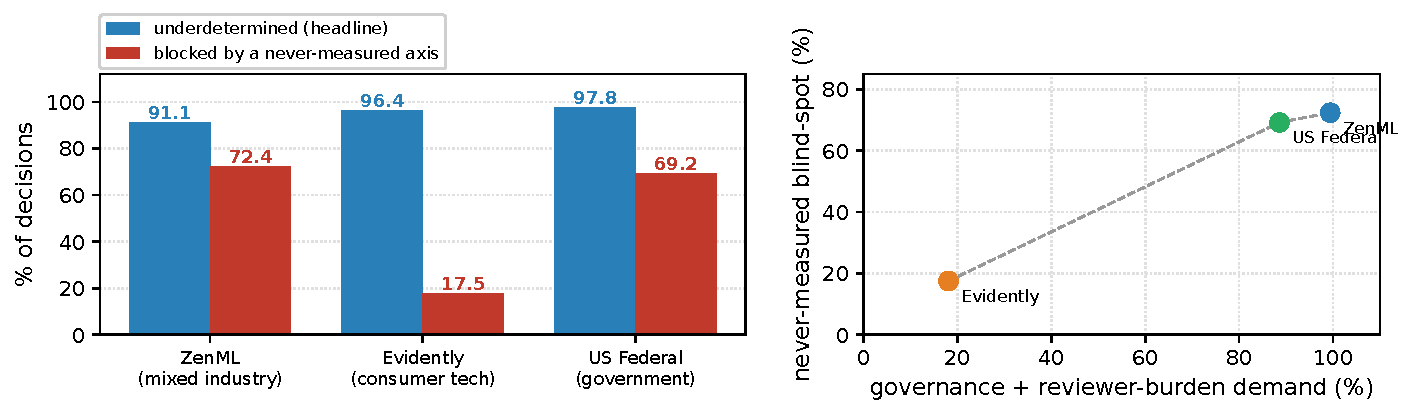
\includegraphics[width=0.74\linewidth]{figures/fig_external_validity.pdf}
\caption{\textbf{The result replicates across three independently-curated corpora; the blind spot scales with demand for never-measured axes.} \textbf{Left:} adversarial-ceiling underdetermination (blue) is robust at $91.1/96.4/97.8\%$ on ZenML (mixed industry), Evidently (consumer tech), and the US Federal AI inventory (government), while the never-measured blind spot (red) varies ($72.4/17.5/69.2\%$). \textbf{Right:} that blind-spot share is near-linear in declared governance$+$reviewer-burden demand---so the variation is the mechanism, not a corpus artifact; the government corpus independently recovers corpus~1's $72.4\%$ on a wholly different population.}
\label{fig:extval}
\end{figure}

\section{The Selective Right-Sizing Procedure}
\label{sec:method}



The map diagnoses; the procedure acts on the diagnosis. For each query it returns exactly one of: \textbf{commit} the identified cheapest-sufficient configuration, when decidable; \textbf{abstain}, when underdetermined---returning the blocking axes \emph{and} an acquisition plan ranking them by $\VoI(a)/\mathrm{acqcost}(a)$, regret reduction per unit measurement cost; or \textbf{infeasible}, when no candidate is feasible in any completion.
$\VoI(a)$ uses the two-world construction of Section~\ref{sec:theory}; by Corollary~\ref{cor:voi} it equals the regret floor of the regime omitting $a$, the implementation matching the closed form to machine precision (Figure~\ref{fig:anchors}, left). Acquisition costs are a documented assumption affecting only the plan \emph{ordering}, never the commit/abstain split (Appendix~\ref{app:acq}). Run blind, the procedure commits on the 8.9\% decidable slice and concentrates its top-ranked measurements on the blocking axes (cost, then reviewer burden and governance).

The two methods that act on an underdetermined verdict---calibrated transfer and the live acquisition loop---are the subject of Section~\ref{sec:resolve}.

\textbf{Risk-tolerant commitment.} Strict decidability is the $\alpha{=}0$ extreme; for a tolerated risk a calibration-based margin enforces $P(\text{infeasible}\mid\text{commit})\le\alpha$, trading coverage against risk (validated on held-out truth, Section~\ref{sec:validation}), whereas the \emph{strict} verdict is indexed instead by which axes carry evidence.

\section{Validation: Deciding Blind Fails; Informed Refusal Pays}
\label{sec:validation}

\begin{figure}[t]
\centering

\includegraphics[width=0.37\linewidth]{figures/fig_hidden_violation.pdf}
\caption{\textbf{Hiding one binding axis: violation rates per slice} (six of the 28 ground-truth slices shown, plus the medium-confidence function-calling slice; full table in Appendix~\ref{app:slices}). Visible-axis ranking (red) and imputation (orange) are \emph{identical} on every slice---filling in the missing value commits the same blind configuration---while the selective procedure (green) abstains and never violates. Pooled over all 28 high-confidence slices ($n{=}476$): 57.1\% vs.\ 0\%, slice-clustered 95\% CI of the gap [46.8, 67.6], McNemar 272/0; 23 of 28 slices are individually significant uncorrected, 15 of 28 after Holm correction.}
\label{fig:hv}
\end{figure}

\subsection{Setup: mask a binding axis, score against the hidden truth}

\looseness=-1 The map cannot by itself show that answering an underdetermined query is harmful, so we test it where ground truth exists. RouterBench supplies per-prompt measured quality and cost for 11 models per benchmark, and fixing one benchmark makes costs comparable. On each of 28 biting slices (17 queries each, 476 pooled decisions; the full slice algebra is in Appendix~\ref{app:slices}) we bind on ground-truth axes, hide one binding axis at the read level (quality, which cheap models trade off, while cost stays visible), and score each rule against the hidden truth. A \emph{hidden violation} is a commitment that violates the hidden constraint. The baselines span practice: \textbf{B2} observed-Pareto, the automated-tooling default that ranks on visible axes and treats the missing one as satisfied; \textbf{B3} median imputation; \textbf{B5} an oracle that sees the hidden axis; and accuracy-only, missing-as-fail, and a cost--quality frontier (B1, B4, B6; Appendix~\ref{app:slices}).

\paragraph{Hidden violations: deciding blind versus abstaining.}
Figure~\ref{fig:hv} and Table~\ref{tab:flagship} give the result. On all 28 slices, B2/B3/B6 commit on 100\% of queries and violate the hidden constraint on 5.9--100\% of them; pooled, \textbf{57.1\%} of their commitments are hidden violations (slice-clustered 95\% CI [46.8, 67.6]). The strict rule abstains on every masked query and so cannot violate; the fair comparison is at \emph{equal final coverage}: the end-to-end pipeline---abstain, measure the named axis, commit---decides all 476 queries with \textbf{zero} violations (Section~\ref{sec:acq}); all 272 paired disagreements against observed-Pareto favor the pipeline (descriptive; the clustered CI is the inference). Per slice, 23 of 28 are significant uncorrected and 15 of 28 after Holm; the pooled clustered result carries the claim (the medium-confidence slice corroborates at 58.2\%; Appendix~\ref{app:slices}).

\looseness=-1 Three readings matter. \emph{Imputation is a no-op}: B3 equals B2 on every slice (a constant fill orders nothing \citep{manski2003partial}); a learned imputer only halves the rate (30.6\%) and the strongest Bayesian rule reaches 4.7\% only by over-provisioning $70\times$, minimum-sufficient on \emph{none} of its commitments (Appendix~\ref{app:reviewer}). \emph{Feasible configs exist} (oracle B5: zero violations everywhere), and \emph{the bite is causal}: violations track Pareto-certified binding exactly (zero off-diagonal over 544 slices; Proposition~\ref{prop:char}).

\looseness=-1 \textbf{What 57.1\% is, and is not.} It is measured on the \emph{quality} axis, a slice-average over a graded spectrum (10\%--93\% across quality floors, across-slice Spearman 0.63; Appendix~\ref{app:reviewer}), not a stable population parameter; the slice-clustered CI carries the inference. \textbf{It does not transfer to governance.} Governance is unmeasured in every configuration-level source by construction, so any governance-binding decision is structurally underdetermined (a decidability claim we verify directly), while the harm \emph{mechanism} is confirmed on a governance-shaped categorical gate at \textbf{16.7\%}--\textbf{53.3\%}---a magnitude set by the gate's admissible-set size, not a measured property of real governance (Appendix~\ref{app:reviewer}). The governance harm \emph{rate} stays unknowable, since no public dataset pairs configurations with governance verdicts (Appendix~\ref{app:audit_data}), and nothing in our argument needs it. The link between the two halves is the binding \emph{mechanism} (Proposition~\ref{prop:char}): an unmeasured binding axis both renders a query underdetermined and, where measurable, makes blind commitment violate---so 57.1\% is a foil, and the informative content is the remedy comparison above, where the selective procedure alone achieves both zero violations and nonzero coverage.

\begin{table}[t]
\centering
\caption{\textbf{Pooled validation on the 28 high-confidence ground-truth slices} ($n{=}476$ masked decisions). HVR = fraction of a rule's commitments violating the hidden binding constraint (entries are proportions). Gap CI: slice-clustered bootstrap (28 clusters); test: one-sided exact McNemar at equal final coverage. B2/B3/B6 coincide per-slice here and share one row; B1 and B4 abstain (B1's ranking axis is the masked one).}
\label{tab:flagship}
\footnotesize
\begin{tabular}{lcccc}
\toprule
Rule & Cov. & HVR & Gap [95\% CI] & McNemar $b/c$ \\
\midrule
B1 accuracy-only $/$ B4 missing-as-fail & 0.00 & 0.000 & --- & --- \\
B2 Pareto $=$ B3 impute $=$ B6 frontier & 1.00 & 0.571 & 0.571 [0.468, 0.676] & 272/0 \\
B5 oracle (sees hidden axis) & 1.00 & 0.000 & --- & --- \\
Selective, strict (ours) & 0.00 & \textbf{0.000} & --- & --- \\
Selective + named measurement (ours) & 1.00 & \textbf{0.000} & --- & --- \\
\bottomrule
\end{tabular}
\end{table}

\subsection{The refusal is informative: the named measurement resolves the decision}
\label{sec:acq}

\looseness=-1 Zero violations at zero coverage would be trivial (B4 achieves it mutely); the value is what the refusal \emph{returns}. With \textbf{two genuine blockers} (quality \emph{and} cost hidden on 510 decisions, neither sufficient alone), the ranked plan resolves every decision in \textbf{2.0} measurements at cost \textbf{0.35} versus \textbf{6.0}/\textbf{2.06} unplanned, every commitment feasible and minimum-sufficient (Appendix~\ref{app:reviewer}).


\paragraph{Risk-tolerant operation.}
Operations may prefer a tolerated risk. The calibrated-margin variant scores against \emph{measured} ground truth (the margin calibrated on a disjoint half, 480/480). The calibration transfers (Figure~\ref{fig:anchors}, right): test feasibility risk \textbf{4.7\%} at \textbf{89.0\%} coverage for $\alpha{=}0.05$ (8.1\% at 92.7\% for $\alpha{=}0.10$). Two honest-boundary caveats---the margin controls \emph{feasibility} risk only, and a held-out prompt split (realized violations $36.6\%\!\to\!14.4\%/3.8\%$)---are in Appendix~\ref{app:prospective}.

\section{Resolving the Gap: Calibrated Transfer and a Live Acquisition Loop}\label{sec:resolve}

Section~\ref{sec:validation} shows that committing blind is unsafe: a point imputer fills every $\bbot$ cell and hides a violation in 53.3\% of decisions. The open question is whether an underdetermined decision can be resolved \emph{without} always paying to measure. We answer it by sorting every underdetermined co-location decision into the \textbf{resolution trichotomy} (Figure~\ref{fig:trichotomy}): a decision is \emph{curable by transfer} when its blocking axis is measurable and predictable from the same model's other benchmarks; \emph{resolvable by measurement} when the axis is measurable but not predictable, so its value must be acquired; or \emph{structurally unmeasured} when no measurement path exists in any public source, as with governance. Algorithm~\ref{alg:resolve} acts on the first two classes in two phases and refuses on the third.

\begin{algorithm}[H]
\caption{Selective Resolution of an underdetermined decision}\label{alg:resolve}
\begin{algorithmic}[1]
\Require query $q$; substrate $S$; conformal radius $\tau_\alpha$; oracle $\mathcal{O}$
\Statex \emph{Phase 1 --- calibrated transfer (no new measurement).}
\For{each fragmented-$\bbot$ quality cell $(x,\text{q})$ blocking $q$}
  \State \textbf{if} axis measurable: belief $\gets[\hat q(x){-}\tau_\alpha,\,\hat q(x){+}\tau_\alpha]$; \textbf{else} skip \Comment{refuse}
\EndFor
\State run verdict; \textbf{if} \textsc{Decidable}: \textbf{commit} cheapest; \textbf{return}
\Statex \emph{Phase 2 --- live acquisition loop (measure what the verdict needs).}
\Loop
  \State $a\gets$ top $\VoI$/cost measurable blocking axis; \textbf{if} none: \textbf{refuse}
  \State \textbf{for} each candidate $x$: belief$(x,a)\gets\mathcal{O}(x,a)$ \Comment{acquire}
  \State run verdict; \textbf{if} \textsc{Decidable}: \textbf{commit}; \textbf{return}
\EndLoop
\end{algorithmic}
\end{algorithm}

\textbf{Phase 1} runs the \emph{unchanged} verdict on a calibrated interval, predicted by leave-one-benchmark-out transfer, rather than a blind point fill. Its guarantee is what makes this safe: the interval is a split-conformal set covering the truth with probability $\ge 1-\alpha$ and a commit fires only when the whole interval clears the threshold, so $P(\text{infeasible}\mid\text{commit})\le\alpha$, finite-sample and distribution-free; on structurally-unmeasured axes it refuses an interval rather than paper over the blind spot. \textbf{Phase 2} spends real measurement only on the axis that most changes the verdict per unit cost, writing it to a scratch overlay that never touches the frozen store, and refuses rather than fabricate a value when only structurally-unmeasured blockers remain.

\begin{table}[h]
\centering
\footnotesize
\caption{\textbf{The trichotomy made quantitative} ($n{=}510$ masked-quality decisions). Coverage is the fraction of underdetermined decisions resolved; HVR the hidden-violation rate among commits. The imputer commits everywhere but blind; transfer trades coverage for a proven safety bound at no measurement cost; the loop buys full coverage with a handful of real probes.}\label{tab:resolve}
\setlength{\tabcolsep}{5pt}
\begin{tabular}{@{}lcccl@{}}
\toprule
Method & Coverage & HVR & Meas.\ cost & Notes \\
\midrule
Point imputation (B2/B3) & 1.00 & 0.533 & 0 & commits blind \\
Calibrated transfer ($\alpha{=}0.05$) & 0.249 & 0.000 & 0 & $P(\text{infeas.}\mid\text{commit})\le\alpha$ \\
Live acquisition loop & 1.00 & 0.000 & 1.0--2.0 probes & min-sufficient 100\% \\
\bottomrule
\end{tabular}
\end{table}

Transfer recovers only about 25\%, a ceiling structural to the decision geometry rather than interval width: the safely-committable decisions are those where a strong model sits far from the threshold, so tightening the interval barely helps (Figure~\ref{fig:frontier}; full sweep and proofs in Appendix~\ref{app:transfer}).

\section{Limitations and Conclusion}
\label{sec:limitations}

\looseness=-1 \textbf{Scope---what this paper does and does not claim.} \emph{Masking simulates missingness} (a live study is next; on never-measured axes our claims are about decidability only); \emph{declared need not bind}---but the certified floor (41.0\%) already assumes \emph{none} does, so granting any binding only raises the rate (\S\ref{sec:map}); and \emph{publication self-selection}---one corpus, though the result replicates on two further independent ones (\S\ref{sec:map})---is the residual external-validity caveat.

\looseness=-1 The finding is a \textbf{certified floor of 41.0\%}, established under the most conservative modelling choices the framework admits, irreducible by better estimates, and robust across three corpora; deciding anyway ships violations only the named measurement prevents. Evidence sufficiency, not estimate quality, is the binding constraint.

\subsubsection*{Reproducibility statement}
All numbers in this paper are regenerated from frozen, versioned artifacts by seeded scripts: the substrate snapshot, the query prior, the decidability map, the masked-validation battery, the VoI identity check, and the guarantee calibration each write a JSON artifact from which the figures and tables are produced verbatim. The code (substrate, solver, validation harness), the frozen snapshot, and the full per-slice tables will be released; determinism is enforced by fixed seeds and tested in CI. The query-derivation taxonomy is released in full (anonymized): the tag list, the tag-to-axis map, the LLM annotation prompts, and the keyword patterns, so the prior is auditable end to end.

\bibliography{references}
\bibliographystyle{iclr2026_conference}

\appendix
\section{Proofs}
\label{app:proofs}

\subsection{Setting for Proposition~\ref{prop:char}}
Fix a query $q=(\tau, c)$, a regime $R$, and the value-reading semantics: each axis of each candidate has a single true value; an in-regime cell reveals its value exactly; an off-regime or unmeasured cell is $\bbot$ and ranges over its admissible domain in a completion. $\cl(R)$ adds to $R$ every axis that is a fixed deterministic function of $R$-axes in the query's context. Assume (i) costs are non-negative with a unique constrained minimizer $x^*(q)$ in the true world, and (ii) every axis domain contains both a value satisfying and a value violating any threshold appearing in $c$ (non-degenerate domains).

\paragraph{Proof of Proposition~\ref{prop:char}.}
\emph{(i) Necessity.} Suppose some $a^* \in \bind(q)$ with $a^* \notin \cl(R)$. Since $a^*$ binds, relaxing its constraint changes the optimum: there exists $x' \neq x^*(q)$ with $\mathrm{cost}(x') \le \mathrm{cost}(x^*(q))$ that satisfies every constraint of $c$ except possibly the one on $a^*$ (if costs tie, the two completions below still disagree on the $\arg\min$, which suffices). Because $a^* \notin \cl(R)$, the cell $(x', a^*)$ is undetermined. Construct two completions that agree everywhere except on $(x', a^*)$: fix every undetermined cell other than $(x', a^*)$ of every candidate with cost at most $\mathrm{cost}(x^*(q))$ at a constraint-violating value---excluding the remaining cells of $x'$ itself, which we fix at satisfying values (possible by non-degeneracy)---fix all other undetermined cells arbitrarily but identically, and set $(x', a^*)$ to a satisfying value in $e_1$ and a violating value in $e_2$. In $e_1$ the optimum is $x'$ (feasible, no costlier than $x^*(q)$, and every cheaper rival is infeasible by construction); in $e_2$ it is $x^*(q)$. Two completions disagree, so $q$ is underdetermined.
\emph{(ii) Sufficiency.} If every axis constrained by $c$ and the cost of every candidate are determined under $\cl(R)$, then no cell that enters any feasibility predicate or the objective is $\bbot$ or straddling; every completion assigns these cells the same (revealed) values, so the feasible set and the $\arg\min$ are identical across $\Comp(E)$, and by uniqueness of the minimizer $q$ is decidable.
The bracket is tight in the stated sense: when the non-binding constrained cells and all costs are determined, the only undetermined cells that can flip the optimum are those on binding axes, so (i) and (ii) coincide. The implementation certifies the sufficient condition for decidability and flags underdetermination only via an explicit witness completion, so flagged queries are provably underdetermined and every reported rate is a floor. \hfill$\square$

\subsection{Proof of Theorem~\ref{thm:floor} and Corollary~\ref{cor:voi}}

\begin{theorem}[Regret floor]
\label{thm:floor}
On the canonical two-candidate family ($x_{\mathrm{cheap}}$ at cost $1$, $x_{\mathrm{safe}}$ at cost $1{+}\delta$, with one binding axis $a^*\notin\cl(R)$ unmeasured for $x_{\mathrm{cheap}}$ and satisfied by $x_{\mathrm{safe}}$), scoring by $L(\hat{x}) = \max(0, \mathrm{cost}(\hat{x}) - \mathrm{cost}(x^*)) + \lambda \mathbf{1}[\hat{x}\text{ violates}]$, any rule restricted to $R$ that must commit one candidate (deterministic or randomized) has worst-case expected regret at least $\Delta = \delta\lambda/(\delta+\lambda)$, and the bound is attained.
\end{theorem}

\begin{corollary}[Value of the missing measurement]
\label{cor:voi}
The value of information of measuring $a^*$---the reduction in minimax committed regret from observing it---equals $\Delta$ exactly.
\end{corollary}

The family has two candidates and two worlds. In $W_{\mathrm{fav}}$, $x_{\mathrm{cheap}}$ satisfies the unmeasured binding constraint, so $x^* = x_{\mathrm{cheap}}$: committing $x_{\mathrm{safe}}$ pays cost overshoot $\delta$, committing $x_{\mathrm{cheap}}$ pays $0$. In $W_{\mathrm{unfav}}$, $x_{\mathrm{cheap}}$ violates, so $x^* = x_{\mathrm{safe}}$: committing $x_{\mathrm{cheap}}$ pays $\lambda$, committing $x_{\mathrm{safe}}$ pays $0$. A rule restricted to $R$ observes identical evidence in both worlds (the only differing cell is off-regime), so its (possibly randomized) action is the same: commit $x_{\mathrm{cheap}}$ with probability $p$. Worst-case expected regret is $\max\{p\lambda,\ (1-p)\delta\}$, minimized where the arms are equal: $p^* = \delta/(\delta+\lambda)$, giving value $\delta\lambda/(\delta+\lambda) = \Delta > 0$, attained by $p^*$. For the corollary: a rule that first measures $a^*$ learns the world and commits its optimum, paying $0$ in each; the reduction in minimax regret from the measurement is therefore exactly $\Delta$. \hfill$\square$

The implemented VoI computes precisely this minimax committed regret by resolving the queried axis both ways while holding other pending axes optimistic; Figure~\ref{fig:anchors} (left) verifies the match at $1.1 \times 10^{-16}$ over $\delta \in [0.05, 1.0]$, $\lambda = 1$, and the released test asserts it at relative tolerance $10^{-9}$ over four $(\delta,\lambda)$ pairs.

\subsection{General regret floor: Theorem~\ref{thm:general}}
\label{app:general}
The two-world family is the $2\times 2$ instance of a general identity. Fix a query, a regime $R$ omitting a binding axis $a^*$, and let the completions of the $\bbot$ cells on $a^*$ induce finitely many \emph{worlds} $j=1,\dots,K$ (each a distinct feasibility/optimum pattern over the $N$ candidates). Define the committed-regret matrix $R_{ij} = \mathrm{cost}(x_i \mid \text{world } j) - \mathrm{cost}(x^*_j)$ if $x_i$ is feasible in world $j$, and $R_{ij} = \lambda_{j}$ (the violation penalty) otherwise; $R_{ij}\ge 0$ and each column has a zero entry (its optimum). A rule restricted to $R$ sees evidence independent of $j$ (only off-regime cells differ across worlds), so its action is a single distribution $x\in\Delta^{N}$ over candidates, with worst-case expected regret $\max_j \sum_i x_i R_{ij}$.

\begin{theorem}[General regret floor]
\label{thm:general}
The minimax committed regret of any rule restricted to $R$ equals the value of the zero-sum game $R$,
\[
V \;=\; \min_{x\in\Delta^N}\max_{j}\ \textstyle\sum_i x_i R_{ij}\;=\;\max_{q\in\Delta^K}\min_{i}\ \textstyle\sum_j q_j R_{ij},
\]
and the value of information of measuring $a^*$ equals $V$ exactly: $\VoI(a^*)=V=\mathrm{EVPI}$, the expected value of perfect information under the least-favorable prior $q^\star$. Theorem~\ref{thm:floor} is the case $N=K=2$, $R=\big[\begin{smallmatrix}0&\lambda\\\delta&0\end{smallmatrix}\big]$, with $V=\delta\lambda/(\delta+\lambda)$.
\end{theorem}

\emph{Proof.} The two expressions for $V$ are equal by the von Neumann minimax theorem (the payoff is bilinear on the product of simplices). A rule restricted to $R$ commits some $x\in\Delta^N$ independent of the world, so its worst-case regret is $\max_j \sum_i x_i R_{ij}\ge V$, with equality at the game-optimal $x^\star$; hence the minimax committed regret is exactly $V$. A rule that first measures $a^*$ learns the world $j$ and commits an $\arg\min_i R_{ij}$ (a zero entry exists in each column), paying $0$; the reduction in minimax committed regret from the measurement is therefore $V-0=V$, i.e.\ $\VoI(a^*)=V$. Finally $V=\max_q\min_i\sum_j q_j R_{ij}$ is, by definition, the largest expected regret a blind committer incurs against any prior $q$ minus the zero regret perfect information attains, i.e.\ the EVPI under $q^\star$. \hfill$\square$

We verify Theorem~\ref{thm:general} numerically (\texttt{run\_general\_voi.py}): the $2\times 2$ corollary reproduces $\delta\lambda/(\delta+\lambda)$ to machine precision ($0$ error over $15$ $(\delta,\lambda)$ pairs), and over $40$ random $N\times K$ instances ($N,K\in[2,6]$) a fictitious-play solver closes the minimax duality gap to $<10^{-4}$ while confirming $V\le$ the regret of every pure blind rule (the floor) and that the independently-computed EVPI matches $V$. A \emph{non-binding} axis---whose completions leave the $\arg\min$ unchanged, a single effective world---has $V=0$: measuring it is worthless, so the VoI is set by the regret geometry (the cost spread and penalty across worlds), never by an estimate of the axis's value. This is why the procedure can rank a governance measurement it cannot impute: $\VoI$ needs the worlds, not the values. We stress that Theorems~\ref{thm:floor}--\ref{thm:general} are elementary (a $2\times2$ zero-sum game and its minimax generalization by von Neumann); their role is to give the implemented VoI a closed-form target to verify against, not to claim a hard theoretical result.

\section{Acquisition-cost table}
\label{app:acq}
The plan ranks blocking axes by $\VoI(a)/\mathrm{acqcost}(a)$ with relative costs grounded in published real-world figures: cost $0.05$ (read a token price sheet, $\approx$ free); latency/throughput $0.10$ and memory/hw $0.20$ (a few GPU-hours of micro-benchmarking, A100 \$0.60--\$4.09/hr, H100 \$1.49--\$6.98/hr); energy $0.15$ (measured by free open-source software---Zeus/NVML/RAPL---piggybacking on the same GPU-time, so \emph{not} a costly axis: we correct an earlier $0.40$); quality $0.30$ (run an eval suite, HELM per-model \$85--\$11k); reviewer burden $0.80$ (sustained expert human review, $\ge$\$40/hr); governance $1.00$ (a SOC\,2 Type\,II audit \$20k--\$80k or a HIPAA assessment \$100k--\$500k+, the most expensive axis by one-to-three orders of magnitude). The two load-bearing facts---price-sheet cost cheapest, compliance audit costliest---hold strongly against real figures. The table affects only the plan ordering; the commit/abstain verdict, the VoI values, and every result in Sections~\ref{sec:map}--\ref{sec:validation} are computed without it, and the $40\times$ perturbation check below confirms the ordering's invariance.

\section{Per-slice validation detail}
\label{app:slices}
The battery auto-discovers every per-benchmark RouterBench slice from the substrate (11 models each; 17 queries per slice at constraint percentiles 10--90), yielding 31 slices of which 29 bite (a slice \emph{bites} when at least one blind-committing baseline violates the hidden truth). The two no-bite slices are reported as no-bite controls and excluded from pooling by construction. Per-slice hidden-violation rates for B2/B3/B6 range 0.059--1.000 and are identical across the three rules on every slice; selective is 0.000 on every slice; B5 (oracle) is 0.000 everywhere, confirming feasible configurations exist on every slice. \textbf{Per-slice significance, stated fully:} one-sided exact McNemar per slice gives $p \in [7.6 \times 10^{-6},\ 0.5]$; 23 of the 28 high-confidence biting slices are individually significant at $0.05$ uncorrected (median per-slice $p = 2.0 \times 10^{-3}$), and 15 of 28 survive Holm correction; the five non-significant slices are small Chinese-language benchmarks where only one or two of the 17 commitments violate. The pooled inference therefore uses the slice-clustered bootstrap (resampling the 28 slices; gap CI [0.468, 0.676]) rather than treating the 476 within-slice decisions as independent, since the 17 thresholds of a slice score the same 11-model pool and are mechanically correlated. The medium-confidence function-calling slice (binding quality and latency, hiding quality, 109 candidates, 17 queries) shows the same pattern (B2=B3=B6 HVR 0.882; selective 0). The latency-masking control on the same family does not bite: cheap function-calling configurations happen to be fast, so the hidden latency floor is co-satisfied and blind commitment is harmless there---the failure mode is specific to hidden axes that cheap configurations trade off, as the binding certification predicts.

\paragraph{Binding certification.}
For every masked query we certify whether the masked axis binds by the active-constraint test (an axis binds iff removing its constraint changes the constrained minimum cost over the ground-truth values). Across all 31 masked slices (527 decisions) plus the 17-decision latency-masking control slice---544 certified queries in total: 287 where the axis binds and blind baselines violate, 257 where it does not bind and they do not, and zero off-diagonal cases. The mis-sizing of Table~\ref{tab:flagship} is therefore attributable to certified binding constraints, not to declared-but-slack ones.

\section{Held-out-sample evaluation}
\label{app:prospective}
To test whether margin-based commitment generalizes beyond the sample it decides on, each slice's prompts are split into a decision sample and a disjoint held-out sample of the same workload (960 scored decisions; this is a prompt split, not a temporal split). Committing by blind cost-minimization violates the constraint on 36.6\% of held-out evaluations; the calibrated-margin selective rule reduces this to 14.4\% at $m{=}0.05$ and 3.8\% at $m{=}0.10$, monotonically in the margin. The min-sufficiency caveat of Section~\ref{sec:validation} applies here equally: the margin buys safety, not minimality.

\section{Confidence-policy and taxonomy ablations}
\label{app:ablations}
\textbf{Confidence policy.} The $\kappa$ sweep is run on the structured grid battery (18 archetype-by-regime cells, thresholds re-grounded per policy). Under $\kappa = \{H\}$ (measured evidence only) underdetermination reaches 100\%: the decidable cases rest on leaderboard-tier (M) cost and latency values. Admitting low-confidence evidence ($\kappa = \{H,M,L\}$) adds no decidability: the additional observations land on axes already populated or already blocked. Underdetermination is never below 89.3\% across the sweep.
\textbf{Taxonomy.} Dropping any single tag-to-axis mapping from the query derivation leaves the ceiling between 83.2\% and 91.1\%; the single largest influence is the human-review mapping ($-7.9$ points), consistent with reviewer burden being a declared constraint in 43.8\% of the documented deployments while unmeasured everywhere.
\textbf{Prior reconstruction.} Uniform prior over constraint patterns: 98.5\% underdetermined (94.2\% attributable to a blind-spot axis). Adversarial governance-light prior (governance and reviewer burden each bound with probability 0.05): 95.7\% (84.5\% attributable). Benchmark-derived prior (constraints proportional to what the corpus measures): 12.4\% (0\% attributable)---the negative control that confirms the mechanism. \textbf{Anti-circularity.} One might worry that underdetermination is tautological: a system that demands axes nobody measures will trivially be underdetermined. The (a)/(b)/(c) decomposition of the 1{,}563 underdetermined decisions refutes this. Type-(a) failures---axes structurally absent from every source (governance, reviewer burden, memory/hw)---account for only \textbf{17.5\%} of underdetermined decisions. The remaining \textbf{82.5\%} are type-(b) \emph{co-location failures}: a measurable axis (cost, latency, quality) has evidence somewhere in the corpus but not for the specific configuration that blocks the query. These are not structural absences; measuring the blocking configuration would resolve them. The system is not simply demanding axes that nobody measures; it is exposing where the evidence that \emph{does} exist fails to co-locate with the configurations that matter.

\begin{figure}[t]
\centering
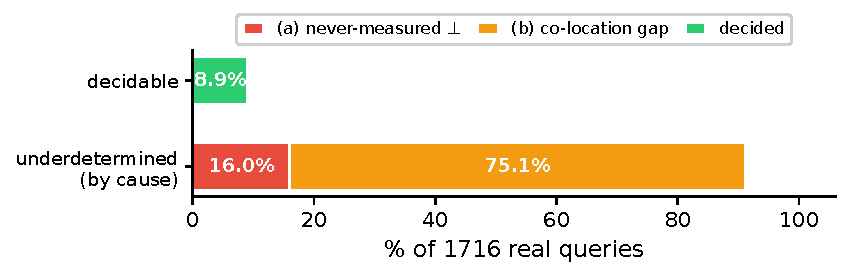
\includegraphics[width=0.62\linewidth]{figures/fig_circularity_decomposition.pdf}
\caption{\textbf{Anti-circularity: 82.5\% of underdetermined decisions are co-location failures, not structural absences.} Each underdetermined decision is attributed to its primary cause: type-(a) a never-measured axis (structural absence, 17.5\%), type-(b) a measurable axis with no evidence for the blocking configuration (co-location failure, 82.5\%), type-(c) an interval straddling the threshold (epistemic uncertainty, 0\%). The finding refutes the circularity concern: the negative-control prior (12.4\% underdetermined) shows the system resolves easily when only measured axes bind; underdetermination arises from measurement gaps, not from demanding the unmeasurable.}
\label{fig:circularity}
\end{figure}

\section{Corpus scale-out}
\label{app:corpus}
Scaling the ingestion pipeline from the five-source measurement snapshot to 20 sources (adding safety, clinical, finance, multilingual, instruction-following, and long-context leaderboards) yields 5{,}164 observations over 655 configurations and 19 archetypes. The three blind-spot axes gain zero observations (per-axis miss rate 1.000 across all 20 sources); the corpus-wide cell miss rate is 0.728, and the measurable axes remain fragmented across sources. Safety and risk leaderboards measure model behavior (e.g., refusal robustness), not deployment governance (e.g., regulatory admissibility of a configuration in a jurisdiction); the gap between those two is exactly the blind spot. The substrate also ships an extraction layer for auto-ingesting paper-reported tables at low confidence with consensus-based promotion; by the confidence-policy ablation above, such evidence cannot alter any hard claim unless explicitly opted into, and no auto-extracted rows are present in the frozen snapshot used here.


\section{Objective masking, verdict sensitivity, plan scoring, and governance bindingness}
\label{app:reviewer}

\begin{figure}[t]
\centering
\begin{minipage}[t]{0.22\linewidth}

\includegraphics[width=\linewidth]{figures/fig_voi_identity.pdf}
\end{minipage}\hfill
\begin{minipage}[t]{0.22\linewidth}

\includegraphics[width=\linewidth]{figures/fig_coverage_risk_gt.pdf}
\end{minipage}
\caption{\textbf{Correctness anchors (implementation checks, not results).} \textbf{Left:} the implemented VoI coincides with the regret floor $\Delta = \delta\lambda/(\delta+\lambda)$ of Theorem~\ref{thm:floor} to machine precision ($1.1 \times 10^{-16}$)---a check that the solver computes the closed form, not a claim about the query distribution. \textbf{Right:} coverage and feasibility risk vs.\ margin $m$, scored on the held-out test half ($n{=}480$ of 960; calibration on the disjoint half); the calibration transfers (4.7\% risk at 89.0\% coverage, $\alpha{=}0.05$).}
\label{fig:anchors}
\end{figure}


\paragraph{Masking the objective (cost).}
The main battery hides quality; here we bind quality and cost at matched percentiles on the same 30 RouterBench per-benchmark slices (510 decisions) and hide \emph{cost} --- the most frequent blocker in the decidability map. The visible-axis rules (observed-Pareto, imputation, cost--quality frontier) rank candidates by visible cost; with the objective unobservable they return no answer on every query (coverage 0): current practice does not silently violate here, it \emph{degenerates}, exactly as the map predicts when the objective axis is $\bbot$ (a constant median fill cannot rank, so imputation degenerates identically). The de-facto fallback --- accuracy-only leaderboard ranking --- commits everywhere and violates the hidden budget cap on \textbf{88.4\%} of commitments (slice-clustered 95\% CI [79.2, 96.1]). The selective procedure abstains and names cost on 510/510 queries; measuring it closes full coverage with zero violations and minimum-sufficient commitments on 510/510 (paired test vs.\ the fallback: 451 disagreements, all favoring the pipeline). One consequence of this setting: the agreement of the three blind rules in Table~\ref{tab:flagship} is a property of two-axis ground truth (they coincide by construction there); under objective masking their behaviors separate (degenerate vs.\ committing fallback).


\paragraph{Learned imputation.}
Pool-median imputation is a constant fill; in the masked-quality setting a genuine training signal exists --- a model's quality on the masked benchmark is predictable from the same model's quality on the other benchmarks. We therefore evaluate the strongest such imputer: leave-one-benchmark-out per-model mean quality, under a per-slice mask that hides quality only for the benchmark under evaluation (so cross-benchmark cells stay visible to the imputer, as they would in practice). Over all 30 slices it cuts the pooled hidden-violation rate roughly in half --- 53.3\% (272/510) for observed-Pareto and median imputation to \textbf{30.6\%} (109/356, clustered 95\% CI [12.9, 30.4]) --- while its coverage drops to 0.70 as the imputed value fails some constraints. Learning helps (paired McNemar 171/8 vs.\ the median fill) but does not repair blind commitment: nearly a third of its commitments still silently violate, with no signal distinguishing them, and on the never-measured axes there is no cross-context signal to learn from at all.

\paragraph{Bayesian expected-regret baseline.}
Point imputation can be replaced by a properly probabilistic rule (the strongest competitor a skeptical practitioner would reach for): per model, fit a posterior $\mathcal{N}(\mu,\sigma)$ over the masked quality axis from the same leave-one-benchmark-out cross-benchmark samples, and among visibly-feasible candidates commit the one minimizing expected feasibility-weighted regret $\mathbb{E}_\theta[\mathrm{cost}(x) + \lambda\,\mathbf{1}(x\text{ violates})]$ (closed-form Normal CDF). Over the 510 masked-quality decisions this drives the hidden-violation rate to \textbf{4.7\%} (24/510) at full coverage --- but only by \emph{over-provisioning}: its commitments are minimum-sufficient on \textbf{0\%} of decisions and cost a mean \textbf{70$\times$} the cheapest-sufficient option (identical at $\lambda{=}1$ and $\lambda{=}4$, so not a penalty-tuning artifact). A Bayesian prior thus trades feasibility violations for gross cost overshoot; it does not recover the cheapest-sufficient configuration, which is the right-sizing target, and on the never-measured axes the posterior collapses to the prior because no cross-context signal exists.

\paragraph{Chance-constrained variant: the wall is the posterior, not the objective.}
One might suspect the $70\times$ overshoot is an artifact of the expected-regret \emph{objective} rather than of partial identification, and that an explicit risk budget would recover minimum-sufficiency. We test the natural alternative: a \emph{chance-constrained} rule (B8) that, under the identical per-model posterior, commits the \emph{cheapest} candidate whose violation probability satisfies $\mathbb{P}(\text{violate})\le\alpha$ (abstaining if none qualifies), swept over $\alpha\in\{0.01,0.05,0.10,0.20\}$. The wall does not move. At $\alpha{=}0.01$ the constraint is unsatisfiable and the rule abstains entirely (0\% coverage); at $\alpha{=}0.05$ and $0.10$ it reaches zero hidden violations but is minimum-sufficient on \textbf{0\%} of commitments, over-provisioning by a mean \textbf{127$\times$} and \textbf{15$\times$} respectively; only at the lax $\alpha{=}0.20$ does any minimum-sufficiency appear (63.5\%), and only by re-admitting hidden violations (16.5\%). \emph{No} $\alpha$ achieves both low violations and minimum-sufficiency: the binding constraint is the width of the posterior over the unmeasured axis---a partial-identification wall---not the choice of objective, exactly as a missing axis (rather than an imprecise one) predicts.

\paragraph{Per-query blocker distribution: the blind spot is not a two-mapping artifact.}
The 72.4\% blind-spot share could in principle be concentrated in the two coarsest taxonomy mappings (governance, reviewer burden). It is not. Reading the complete blocking set of each of the 1{,}563 underdetermined queries, the mean blocker-set size is \textbf{2.3} (multiplicity is the norm: 360 queries blocked by one axis, 519 by two, 495 by three, 189 by four or five). Cost is the modal blocker---present in \textbf{82.5\%} of underdetermined queries and the \emph{sole} blocker in 9.7\%---while governance is present in 61.0\% but sole in only \textbf{4.7\%}, and reviewer burden present in 48.0\% but sole in \textbf{8.6\%}. Only \textbf{17.5\%} of underdetermined queries have a blocking set contained in $\{$governance, reviewer burden$\}$ (the queries that deleting both mappings could resolve); the other \textbf{75.1\% of all queries} survive on a different blocker---reconciling exactly with the joint-drop floor---and the independent never-measured-axis cross-check recovers the published \textbf{72.4\%}. Two coarse mappings therefore do not carry the result; the blind spot is distributed across axes, with cost the most frequent contributor.

\paragraph{Proxy harm validation on a categorical governance-like axis.}
The pooled 57.1\% harm is on the \emph{continuous} quality axis, whereas the result is driven by governance---a \emph{categorical} admissibility gate. To bridge the gap we construct such a gate over the eleven RouterBench models: open-weights / self-hostable models (the six \texttt{meta-*}, \texttt{mistralai-*}, \texttt{wizardlm-*}, \texttt{zero-one-ai-*}) are \emph{admissible} under a data-sovereignty governance constraint (``data may not leave a self-hosted boundary''); the five proprietary-API models (\texttt{claude-*}, \texttt{gpt-*}) are not. Admissibility here is a \emph{verifiable licensing fact}, not an invention: Mistral/Mixtral ship under Apache-2.0, Llama-2/Code-Llama/WizardLM under the Llama 2 Community License, Yi-34B under Apache-2.0---all self-hostable; Claude and GPT release no weights and run only on the provider's servers. It is a clearly-labelled \emph{validation} ground truth---never written to the substrate---exactly as RouterBench quality is the hidden truth in the masked-quality battery. We bind \emph{quality $\ge$ percentile} \emph{and} \emph{self-hostable}, mask the gate at the read level, let each blind rule commit on visible quality and cost, and score against the hidden gate (a hidden violation $=$ committing a proprietary model under a self-hosting requirement). Over 270 query instances (30 slices $\times$ 9 quality floors) blind commitment (B2/B3/B6, identical) violates the categorical gate on \textbf{16.7\%} of decisions (G1, self-hostability / data-sovereignty), and the bite is \emph{graded by the quality floor} exactly as for the continuous axis: $0\%$ at the p10--p30 floors (the cheapest quality-feasible model already self-hosts), rising through $20.0\%$ (p60), $26.7\%$ (p70), $43.3\%$ (p80) to \textbf{53.3\%} at p90---where a high quality floor forces a proprietary model and the self-hosting requirement is silently broken, in line with the 57.1\% on quality. An admissible config exists on $229/270$ instances, where the oracle and the selective+measurement pipeline commit with \emph{zero} violations (McNemar $45/0$); the remaining $41$ are genuinely infeasible (no self-hostable model clears the floor), where even the oracle abstains.

\emph{Multi-gate robustness.} To rule out a single-gate artifact, we repeat the battery under two further independently-defined categorical gates over the same 150-instance pool: G2 (EU data-residency / GDPR: open-weights and GPT qualify; Claude models do not, lacking a documented Anthropic EU data centre as of the corpus date) yields HVR $= \mathbf{8.0\%}$; G3 (commercial fine-tuning rights: Apache-2.0 models only, i.e.\ Mistral-7B and Mixtral-8x7B) yields HVR $= \mathbf{45.3\%}$, the higher rate reflecting only two admissible models. Blind-commit harm holds across all three gates (min HVR $= 8.0\%$), ruling out the single-gate artifact concern. We read $\min(\text{HVR}) = 8.0\% > 0$ as the \emph{mechanism} claim---blind commitment harms regardless of which governance gate is operative---and stress that the \emph{magnitude} ($8.0\%$--$45.3\%$) is a function of each constructed gate's admissible-set size (2/11 for G3 vs.\ 8/11 for G2), not a measured property of real governance, which stays unmeasured. The categorical gate is a bridge that the harm mechanism operates on a governance-shaped constraint, not an estimate of real governance harm. To our knowledge, this is the first harm validation on hard categorical, governance-shaped constraints. The constraint and its admissibility set are real (data sovereignty is a documented enterprise requirement, and self-hostability is fixed by each model's license); what we supply is the decision to test \emph{this} governance constraint, since no source pairs configurations with audited governance outcomes.

\textbf{Relationship to practitioner knowledge.} A practitioner who knows their governance constraint applies it manually and never commits a violating config---precisely what our oracle baseline (B5) models, which achieves 0\% violations in all three gates. The 8.0\%--45.3\% harm arises in the blind-commit rules (B2/B3/B6) that treat the governance axis as either satisfied or unknown. This is the empirically relevant case: governance constraints are genuinely unmeasured in every public source (§\ref{sec:map}), so a practitioner cannot apply them manually without first running an audit (whose cost VoI ranks). The masked-quality battery uses the same convention (missing quality treated as satisfied in B2) for the same reason: it models the deployer who has not yet acquired the missing measurement.

\paragraph{Declared-versus-binding sensitivity (binding probability $p$) and measured anchors.}
On the axes that drive the result we assume a declared constraint binds at the optimum, which is unverifiable where the axis is unmeasured. We replace the binary assumption with a sensitivity: keep each declared governance / reviewer-burden binding (tag-derived and the regulated-industry rule) with probability $p$, reclassify all 1{,}716 queries, and sweep $p$. Under full-domain completion the rate is monotone in $p$: \textbf{75.1\%} ($p{=}0$, reproducing the skeptic floor), $80.4\%$ ($p{=}0.25$), \textbf{84.3\%} ($p{=}0.5$), $88.2\%$ ($p{=}0.75$), \textbf{91.1\%} ($p{=}1$, reproducing the adversarial ceiling); the blind-spot-attributable share moves $1.2\% \to 30.5\% \to 50.3\% \to 63.3\% \to 72.4\%$ in step. The finding therefore does not rest on the strong declared-implies-binding assumption: even if only half of declared governance/reviewer constraints actually bind, five-sixths of decisions remain underdetermined.

Three external anchors bracket the plausible $p$ range.
(i)~\emph{Explicit-binding LLM test} (Qwen2.5-32B-Instruct $\times$ 3 prompt variants, bfloat16 on H100): of 980 governance-tagged case studies, only 1 receives a BINDING majority label ($\hat{p}_{\text{32B}} \approx 0.001$). This reflects the nature of the texts---engineering case studies describe solutions built, not governance constraints imposed; binding requirements are rarely stated explicitly in the narrative. This is a strict lower bound.
(ii)~\emph{Keyword extraction} for binding-indicating phrases (self-hosting mandates, external-API prohibitions, data-sovereignty clauses): $\hat{p}_{\text{kw}} = 7.5\%$ (72/954), a conservative explicit floor.
(iii)~\emph{US Federal AI Inventory} (OMB 2025, $n{=}1{,}290$ GenAI use cases), self-reported governance binding-\emph{indicator} fields: $\hat{p}_{\text{OMB}} = 34.5\%$ (445/1{,}290; ATO dominant at 25.4\%). This anchor records a \emph{declared} requirement, not activeness at the optimum, and is the highest of the three.
All three---and every $p$ in the range $[0.001, 0.345]$---fall within the published $75.1\%$--$91.1\%$ sweep envelope. The finding is robust to the binding assumption: even at $p = 0$ (zero governance binding) the rate is $75.1\%$, well above three-quarters. The $p$-sweep is retained as a sensitivity analysis; the three anchors provide grounded reference points within it.

\paragraph{On minimum-sufficiency as the target.}
We score against the \emph{cheapest sufficient} configuration, and the Bayesian and chance-constrained rules' $70\times$/$127\times$ overshoots are failures \emph{relative to the stated constraint}. A risk-averse deployer who deliberately over-provisions (headroom, future load, vendor consolidation) is not in conflict with this: deliberate headroom is a \emph{different, explicit} requirement, expressed by raising the stated constraint (a higher quality floor, a latency margin), after which right-sizing targets the cheapest configuration sufficient \emph{for that} requirement. What the framework flags as a failure is over-provisioning that is \emph{not} a stated requirement but an artifact of being unable to identify the sufficient configuration---paying $70\times$ because the evidence cannot tell you which cheaper option suffices, not because you chose headroom. Minimum-sufficiency relative to the true requirement is thus the right target by construction; the over-provisioning we penalize is the one no deployer asked for. (Relatedly, the operative quality percentile in the masked-quality battery is not our free parameter but the \emph{deployment's declared floor}; the graded-bite sweep, $10\%$ at p10 to $93\%$ at p90, brackets every choice a deployment could make.)

\paragraph{Joint-drop and strict-binding rate variants.}
Single-mapping deletions cannot detect correlated overcounting, and a declared constraint is not a certified binding one. Reclassifying all 1{,}716 queries through the identical path: deleting the governance \emph{and} reviewer-burden mappings simultaneously (tags and the industry rule) leaves \textbf{75.1\%} of decisions underdetermined; restricting governance to bind only on the 73 case studies whose text contains explicit candidate-excluding language leaves \textbf{87.3\%}; applying both restrictions leaves \textbf{75.9\%}. Under the most conservative reading the taxonomy admits, three quarters of real decisions remain underdetermined, and the modal blocker becomes cost --- a measurable axis whose evidence is simply absent from most candidate pools. The 91.1\% adversarial ceiling is therefore an upper reading of a quantity whose skeptic floor, under maximal skepticism about declared governance, is still roughly 75\% (and whose certified floor, additionally bounding the measurable axes, is 41.0\%).

\paragraph{Cost-versus-structural decomposition of the ceiling.}
Cost, though frequently $\bbot$ in a candidate pool, is cheaply acquirable (price-sheet arithmetic, acquisition cost 0.05) and so is not a true structural blind spot like governance. We decompose the 1{,}563 underdetermined decisions by their complete blocking set and ask what survives \emph{granting cost as determined} (Figure~\ref{fig:costdecomp}). On the adversarial ceiling, only \textbf{8.9\%} of all decisions are cost-only (resolved by granting cost); \textbf{82.2\%} remain underdetermined with a non-cost blocker --- \textbf{72.4\%} of all decisions on a never-measured axis (the structural core), 9.8\% on another co-located measurable axis --- with the structural-only share (16.0\%) a hard floor on this. On the joint-drop (skeptical-floor) prior the picture inverts: granting cost resolves \textbf{38.2\%}, and the residual structural share is only 1.2\%. The 91.1\% adversarial ceiling is therefore structural (granting cost barely moves it); the 75.1\% skeptic floor is what leans on cost, because that reading first deletes the never-measured governance and reviewer-burden bindings. Two further readings confirm the split. A fully \emph{governance-agnostic} prior---binding only measurable axes, with no never-measured axis able to bind at all---still leaves \textbf{75.1\%} underdetermined, by construction entirely cost and measurable co-location (granting cost on top still leaves 36.5\% from co-location alone). The \emph{strict-joint} prior (governance restricted to the 73 keyword-explicit cases, reviewer burden dropped) leaves 75.9\%, of which only \textbf{5.3\%} is structural---that keyword-explicit governance---and the rest is cost and co-location.

\begin{figure}[h]
\centering
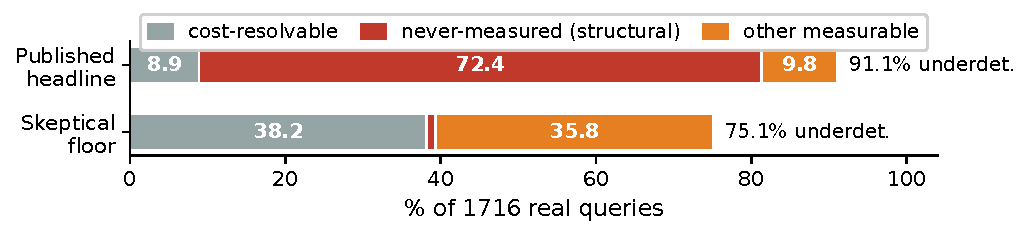
\includegraphics[width=\linewidth]{figures/fig_cost_decomposition.pdf}
\caption{\textbf{The ceiling is structural; the skeptic floor leans on cost.} Each bar decomposes the underdetermined decisions (as \% of all 1{,}716 queries) by what survives \emph{granting cost as determined}: the share cost alone resolves (grey), the residual blocked by a never-measured axis (red), and the residual blocked by another measurable axis (orange). On the \emph{adversarial ceiling}, granting cost resolves only 8.9\% while 72.4\% remain blocked by an axis no source measures---the cause is not cost co-location. On the \emph{skeptic floor} (governance and reviewer-burden bindings deleted), granting cost resolves 38.2\% and the structural residual is 1.2\%, so it is the floor, not the ceiling, that rests on cost.}
\label{fig:costdecomp}
\end{figure}

\paragraph{Graded bite: violation rate versus trade-off strength.}
The no-bite control (Appendix~\ref{app:slices}) is binary; here we make it continuous (Figure~\ref{fig:gradedbite}). Per slice we score the \emph{trade-off strength} as the Spearman correlation between a config's true cost and its true quality (positive $\Rightarrow$ cheaper configs are lower-quality $\Rightarrow$ committing the cheapest tends to violate a quality floor). Across the 30 slices the blind-commit violation rate rises smoothly with it (Spearman \textbf{0.63}): from \textbf{29.4\%} in the weak-trade-off tercile, through 48.2\%, to \textbf{82.3\%} in the strong tercile. The complementary view---violation rate against the quality-constraint percentile---is monotone from \textbf{10\%} at p10 to \textbf{93\%} at p90. The pooled 57.1\% is thus a slice-average over a graded spectrum, with the no-bite control at the weak-trade-off end, not an artifact of a binary cliff.

\begin{figure}[h]
\centering
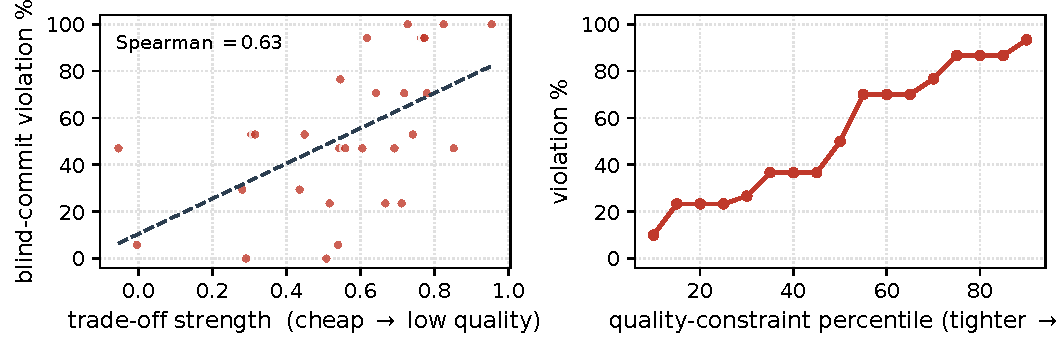
\includegraphics[width=\linewidth]{figures/fig_graded_bite.pdf}
\caption{\textbf{The bite is graded, not binary.} \textbf{Left:} per-slice blind-commit violation rate versus trade-off strength (Spearman correlation between a config's cost and quality; higher $\Rightarrow$ cheaper configs are lower-quality); the rate rises with it (across-slice Spearman 0.63), with the no-bite regime at the weak-trade-off end. \textbf{Right:} violation rate versus the quality-constraint percentile, monotone from 10\% (lenient) to 93\% (strict). The pooled 57.1\% averages over this spectrum.}
\label{fig:gradedbite}
\end{figure}

\paragraph{Cost-threshold sensitivity of the floor.}
Because cost is the floor's modal blocker, we re-ground its threshold across percentiles \{p25, p40, p50, p60, p75\} (other axes fixed at p50) on the joint-drop prior: the floor is \textbf{bit-identical at 75.1\%} throughout. As with the main result, the verdict turns on whether an axis carries evidence at all, not on where a threshold sits.

\paragraph{Corpus composition (deleting whole industries).}
The published prior robustness re-weights the query distribution within the single corpus; this tests the complementary axis --- whether the result depends on \emph{which} deployments populate it --- by deleting entire industries and re-running the identical classifier (only the row set changes). Deleting all five regulated industries (Healthcare, Finance, Legal, Insurance, Government), the sub-population that drives governance binding, leaves \textbf{88.8\%} of the remaining 1{,}360 decisions underdetermined (modal blocker cost); deleting the dominant Tech majority (904 rows) leaves \textbf{96.8\%} of 812. Within each industry of $\ge 30$ rows the rate ranges 86.0\% (Tech) to 100\% (Finance, Healthcare, Legal --- governance-modal there), and every leave-one-industry-out complement stays in 90.0--96.8\%. In every partition cost remains the modal blocker. This establishes composition robustness within the corpus; the independent second corpus below addresses the cross-corpus question directly.

\paragraph{External-validity replication on two independent corpora.}
To test the strongest external-validity worry---publication self-selection in a single corpus---we replicate on two \emph{separately curated} corpora, deriving queries under the \emph{same} semantics (documented, deliberately conservative cross-vocabulary maps) and running the \emph{identical} classifier against the \emph{same} frozen substrate. \textbf{Corpus 2} is the Evidently AI ML/LLM system-design database (MIT mirror, commit pinned; \textbf{502} LLM deployments curated by a different maintainer than ZenML), consumer-tech-skewed. \textbf{Corpus 3} is the US Federal AI Use Case Inventory (OMB, public domain; \textbf{1{,}290} GenAI use cases self-reported by federal agencies under EO~13960)---US public-sector, the opposite skew. The result replicates on both and slightly exceeds: \textbf{96.4\%} and \textbf{97.8\%} underdetermined (vs.\ 91.1\%), so ``most right-sizing decisions are unidentified'' is not a ZenML artifact. The blind-spot \emph{composition} then \emph{brackets} exactly as the mechanism predicts. Corpus 2 declares governance/reviewer burden rarely (13.8\%/4.4\%, vs.\ 55.6\%/43.8\% in corpus 1), so its underdetermination is cost-driven and only \textbf{17.5\%} is blind-spot-attributable; corpus 3, being government, declares them heavily (28.9\%/59.7\%) and its blind spot is \textbf{69.2\%}---\emph{independently recovering corpus 1's 72.4\%} on a wholly different population. Across three maximally different corpora the result is robust, and the governance-attributed fraction scales with governance demand, confirming the mechanism rather than a corpus artifact (Figure~\ref{fig:extval}). Importantly, the OMB corpus records governance requirements as \emph{structured machine-readable fields} (authority-to-operate, PII flag, high-impact designation) independently of the deployed solution---it answers what constraints are \emph{declared}, not what was built---and still shows $97.8\%$ underdetermination and a $\hat{p}_{\text{OMB}} = 34.5\%$ binding-indicator rate, confirming the mismatch is not an artifact of deployment-description corpora.


\paragraph{Verdict sensitivity.}
Re-running the full 1{,}716-query map at FULL regime: the underdetermination count is \textbf{bit-identical (1{,}563/1{,}716 = 91.1\%)} under every threshold-grounding percentile in \{p25, p40, p50, p60, p75\} and under a relative cost-tie tolerance $\varepsilon \in \{0, 0.01, 0.05, 0.10, 0.20\}$ (a rival flips the $\arg\min$ only when it could undercut the best sure option by more than $\varepsilon$; $\varepsilon{=}0$ cross-checks bit-identical against the published classifier on all 1{,}716 queries). The verdict is driven by which axes carry evidence at all, not by threshold placement or tie-breaking --- consistent with 72.4\% of queries being blocked by a corpus-wide-$\bbot$ axis.

\paragraph{Completion-semantics sensitivity.}
The criterion completes each $\bbot$ cell over its \emph{entire} domain --- the conservative reading that makes every rate a certified lower bound, but also an adversarial one. Confining $\bbot$ cells on the measurable axes (quality, cost, latency) to their observed corpus range instead --- a \emph{bounded-prior} reading, queries and thresholds unchanged, under interval semantics --- lowers the rate from the full-domain \textbf{91.1\%} to \textbf{56.9\%}, and this is \emph{robust to the bound width}: a point ($p50$), $[p40,p60]$, $[p25,p75]$, and $[p10,p90]$ all give 56.9\%. So roughly a third of the full figure is the adversarial-completion tail on the measurable axes; the \textbf{56.9\%} that survives \emph{any} bounded belief is the criterion-robust core, of which \textbf{47.3} points are blocked by a never-measured axis --- which admits no bounded range at all, there being no evidence to bound it with. We read 91.1\% as the adversarial ceiling and 56.9\% as its any-reasonable-belief floor. (Relatedly, the three-valued verdict's \emph{infeasible} label is empirically empty here: \textbf{0/1{,}716} queries are infeasible, so the binding question is always decidable-versus-underdetermined, never ``no feasible candidate exists.'') Operationally, what a deployer can cheaply acquire sets the relevant floor: under price-sheet (cost) access the irreducible remainder is the structural residual, whereas 75--91\% is what the evidence \emph{as published} leaves before any acquisition. We note that the procedure can still \emph{rank} a measurement on such a never-measured axis: its VoI is the two-world regret (Section~\ref{sec:theory}), which needs the cost spread and violation penalty, not an estimate of the axis's value---so a governance measurement is ranked precisely where imputation, lacking any cross-context signal, has nothing to compute.

\paragraph{Scoring the acquisition plan under two genuine blockers.}
Hiding quality \emph{and} cost simultaneously on the same 510 decisions makes the blocking set $\{$quality, cost$\}$ on every query, and a necessity ablation confirms neither measurement alone resolves any of them. Following the procedure's ranked plan (re-ranked after each reveal) resolves every query in exactly \textbf{2.0 measurements} at cumulative acquisition cost \textbf{0.35} (the plan names cost first on 510/510, as the VoI-per-cost ordering implies); revealing uniformly random axes until commitment needs \textbf{6.0 measurements} and cost \textbf{2.06} on average. Every plan-final commitment is feasible and minimum-sufficient against ground truth (510/510).

\paragraph{Acquisition-cost-table sensitivity of the plan.}
The plan's efficiency is invariant to the (assumed) acquisition-cost table. Across perturbations --- cost $\times 5$, cost $\times 20$ (dearer than quality), quality cheap, all axes equal, and per-axis random $\times[0.5, 2]$ --- the plan resolves in \textbf{2.0} measurements versus \textbf{6.0} random, names cost first on \textbf{100\%} of decisions, and stays feasible and minimum-sufficient on \textbf{100\%}. Both genuine blockers must be revealed to commit, so the plan's count is structural; cost is named first because its VoI dominates, not because the table makes it cheap to acquire --- so the ordering, contrary to the worry that it ``depends entirely on the cost table,'' survives a $40\times$ swing in that table here.

\paragraph{Candidate-discriminating governance language.}
A conservative keyword scan of the 954 governance-tagged case studies (patterns listed in the released script; matches require language tying a regulatory/privacy requirement to a configuration choice) finds \textbf{72 (7.5\%)} with explicit candidate-discriminating governance language --- a floor, since paraphrases escape keyword patterns. Named examples where governance changed the deployment decision: \textbf{QuantumBlack} (drug discovery) ``could not leverage API-based models like GPT-4'' and chose a self-hosted alternative; \textbf{John Snow Labs} (healthcare) ``couldn't use general-purpose LLMs like GPT-4'' and deployed domain-specialized models; \textbf{Slack} ``cannot send data to third-party'' and built private infrastructure; \textbf{Qatar Computing Research Institute} ``cannot simply use cloud-based LLM'' and deployed on-premises. In each case a cheaper or higher-quality external option was excluded, confirming governance binds at the optimum. Other examples: a legal-tech deployment whose client data ``cannot sit on third-party'' infrastructure; a finance deployment routing all LLM traffic through a self-hosted proxy for ``full data sovereignty''; a pharma deployment selecting self-hosted open-source models for regulatory reasons; an enterprise case stating compliance requirements ``significantly constrain architectural choices and often favor private'' deployment. Declared governance therefore excludes concrete candidates in at least a non-trivial fraction of documented deployments; whether it binds at the optimum in each case remains unverifiable precisely because the axis is unmeasured --- the paper's central point. As measurement units we envision deployer-side artifacts: a governance observation as an audit outcome per (configuration, jurisdiction), reviewer burden as human-minutes per output from a pilot, published to compliance registries (model-card or conformity-documentation style) rather than to leaderboards.

\paragraph{The two modelling knobs (detail for Table~\ref{tab:twobytwo}).}
The $2\times2$ in Section~\ref{sec:map} fixes the rate by two orthogonal choices: the completion of a $\bbot$ cell on a \emph{measurable} axis (full-domain, each cell ranging over its entire admissible domain---the most adversarial reading---versus bounded to the corpus-observed range), and whether a \emph{declared} governance/reviewer-burden constraint is granted as binding ($p{=}1$) or deleted ($p{=}0$). Every cell is a witness-based lower bound within its semantics (the sense in which each rate is ``at least''). The assumption-minimal corner---bounded completion \emph{and} no declared binding---is \textbf{41.0\%}, stable across bound widths (point-$p50$, $[p25,p75]$, $[p10,p90]$ all give 41.0\%) and only 0.5 pp structural-attributable. Sweeping the binding probability $p$ under bounded completion is monotone---41.0\% ($p{=}0$), 48.1\% ($p{=}0.345$, the OMB anchor), 56.9\% ($p{=}1$)---so each added assumption is a quantified increment between the floor and the ceiling.

\paragraph{Publication self-selection: direction of the bias.}
The query prior is built only from companies that publish deployment case studies, which is the paper's key external-validity limitation. We argue the resulting bias plausibly \emph{favors} the finding rather than against it, by a measurement-maturity mechanism: teams that publish case studies are disproportionately the better-resourced, better-instrumented ones---they ran the quality, cost, and latency evaluations that make a case study worth writing. If anything, the published corpus \emph{over}-represents well-measured deployments, so the unpublished tail is plausibly \emph{less} instrumented on exactly the measurable axes, leaving \emph{more} of its decisions underdetermined, not fewer. The blind-spot axes (governance, reviewer burden) are unmeasured everywhere regardless of publication, so self-selection cannot deflate them. This is an argument, not a second-corpus validation, which remains the irreducible open limitation.

\paragraph{Noisy measurement.}
The framework as stated assumes a measurement reveals an axis's value (an interval or a point); a governance audit returning \emph{probabilistic} admissibility is not yet modeled. The possible-worlds machinery extends naturally---a noisy measurement \emph{narrows} the completion set rather than collapsing it to a singleton, so a query can stay underdetermined after measuring if the residual completions still disagree---but the calibration of that residual, and a value-of-noisy-information that accounts for it, is future work. This matters most for precisely the axes we care about, where measurement is itself uncertain; we flag it as a scope boundary rather than claim it.

\paragraph{When cheap configurations happen to co-satisfy a hidden axis.}
On the masked-validation slices, blind commitment violates the hidden constraint on $57.1\%$ of decisions, so on the complementary $\approx 42.9\%$ the cheapest visible configuration \emph{happens} to satisfy the hidden axis. This co-satisfaction shrinks the realized harm in any particular deployment---but it is luck the decider cannot see ex ante, since the axis is unmeasured: the same blind rule that wins on the $42.9\%$ loses on the $57.1\%$, with no signal to tell the two apart. The selective procedure's value is exactly that it does not gamble on the co-satisfaction it cannot observe.

\paragraph{Operational value when the top blocker is a single expensive measurement.}
The VoI ranking is most useful when several cheaply-measurable blockers must be triaged; when the binding axis is a never-measured one with a single expensive measurement path (a governance audit), the ranking's marginal value over ``run the audit'' is smaller. What the procedure still contributes there is \emph{decision discipline}: it certifies that the decision is genuinely unidentified (not merely imprecise), names the audit as the resolving measurement and prices it against the two-world regret floor, and---critically---declines to ship a confident-looking blind commitment that imputation would have produced. For a regulated deployer who already runs audits, the contribution is the certificate that no cheaper evidence substitutes for one.

\paragraph{Experiment-to-$n$ map.}
Table~\ref{tab:nmap} lists each experiment, its sample size, and what it tests, to make the slice algebra in Section~\ref{sec:validation} and the result robustness checks traceable at a glance.

\begin{table}[h]
\centering
\caption{\textbf{Each experiment, its $n$, and what it tests.} ``Queries'' are right-sizing decisions derived from documented deployments; ``masked decisions'' are RouterBench ground-truth slices with one binding axis hidden.}
\label{tab:nmap}
\footnotesize
\setlength{\tabcolsep}{4pt}
\begin{tabular}{lll}
\toprule
Experiment & $n$ & What it tests \\
\midrule
Decidability map (Sec.~\ref{sec:map}) & 1{,}716 queries & ceiling underdetermination at full evidence \\
Cost-vs-structural decomp.\ (App.) & 1{,}563 underdet.\ & blind spot structural, not cost co-location \\
Per-query blocker dist.\ (App.) & 1{,}563 underdet.\ & not a two-mapping artifact (Q4) \\
Completion-semantics sweep (App.) & 1{,}716 queries & range $56.9$--$91.1\%$ across belief width (Q1) \\
Declared$\Rightarrow$binding sweep (App.) & 1{,}716 queries & ceiling monotone in binding prob.\ $p$ (W2) \\
Corpus composition (App.) & 1{,}716 queries & robustness to indexed industries \\
Masked validation, pooled (Sec.~\ref{sec:validation}) & 476 masked & blind commitment violates; abstain does not \\
Full slice algebra (App.) & 527 (510 truth) & per-slice violation, bind certification \\
Bayesian / learned / B8 (App.) & 510 masked & probabilistic rules over-provision (Q2) \\
Graded bite (App.) & 30 slices & violation rate vs.\ trade-off strength \\
Categorical-gate harm (App.) & 270 masked & blind commit violates self-hosting gate (W3) \\
Independent-corpus replication (App.) & 502 $+$ 1{,}290 & ceiling $96.4\%/97.8\%$ on two corpora (W4) \\
General regret floor (App.) & 40 games & minimax identity $=$ VoI (Thm~\ref{thm:general}) \\
Acquisition plan, two-blocker (Sec.~\ref{sec:acq}) & 510 masked & 2.0 vs.\ 6.0 probes; min-suff.\ commits \\
Calibrated-margin guarantee (Sec.~\ref{sec:validation}) & 480/480 split & held-out risk, $4.7\%$ at $89\%$ cov.\ \\
\bottomrule
\end{tabular}
\end{table}


\section{Measured Declared$\to$Binding Rate (Experiments A1--A3)}
\label{app:binding_rate}

These three experiments provide external anchors for the declared$\to$binding probability $p$ used in the sensitivity sweep of Appendix~\ref{app:reviewer}.

\paragraph{What these anchors measure, and what they do not.} A boundary governs every experiment here. We use the annotators (LLMs, keywords, OMB fields) to read what a deployment \emph{declares}---whether its narrative states a governance requirement that excludes a concrete candidate configuration. We do \emph{not} use them to predict whether governance \emph{truly} binds at the optimum: that would require the admissibility value of the unmeasured axis itself, exactly the imputation our framework forbids. The distinction is operational, not rhetorical: these labels anchor the prior probability $p$ in the declared$\to$binding sweep (Appendix~\ref{app:reviewer}); they are \emph{never} written to the substrate, never fill a $\bbot$ cell, and never enter a decidability verdict. Reading a declared constraint is a text-classification task an LLM is suited to; predicting an unmeasured value is the label-substitution that \citet{dorner2025limits} prove cannot succeed---and which our never-impute stance refuses on principle. So a low binding rate or low inter-annotator agreement is not a failure of the method: it is direct evidence that binding is \emph{rarely stated explicitly} in these narratives, which is itself why the axis must be measured rather than inferred.

\subsection*{A1 — Multi-LLM Ensemble Annotation}
To make the reliability proxy \emph{inter-model} agreement rather than single-model intra-prompt agreement, we annotate the $n{=}980$ governance-tagged ZenML case studies (industries in REGULATED $\cup$ governance tags) with an ensemble of three instruct models from three different providers---\textbf{Qwen2.5-32B-Instruct} (Alibaba), \textbf{Meta-Llama-3-8B-Instruct} (Meta), and \textbf{Mistral-7B-Instruct-v0.3} (Mistral)---so their training biases are not shared. Each model uses the same 3 prompt variants and rubric (majority vote within model, then majority vote across the three model-labels; ties $\to$ UNDETERMINED). Labels are BINDING / NON\_BINDING / UNDETERMINED, classifying the \emph{declared} text per the boundary above.
Per-model binding rate: $\hat{p}_{\text{Qwen}} = 0.1\%$, $\hat{p}_{\text{Llama}} = 0.4\%$, $\hat{p}_{\text{Mistral}} = 1.1\%$; \textbf{ensemble} $\hat{p}_{\text{LLM}} = 0.2\%$ (2/980; 95\% CI $[0.0\%, 0.5\%]$), inter-model Fleiss $\kappa = 0.096$.
\emph{Interpretation.} The ZenML corpus consists of engineering case studies describing solutions built, not governance constraints imposed; a candidate-excluding governance mandate is rarely stated explicitly in the narrative, so most cases (974/980) are classified UNDETERMINED across all three providers. Raw inter-model agreement is in fact high---pairwise $95.6\%$--$98.1\%$, and all three models agree on $95.0\%$ of cases; the low Fleiss $\kappa$ is the prevalence paradox, deflated because one category dominates, not a sign of disagreement. That three models from three providers independently find binding almost never \emph{declared} is the substantive result: it is direct evidence the axis must be measured, not inferred from text. The ensemble rate is a strict lower bound on declared binding: $\hat{p}_{\text{LLM}} \approx 0.2\% \Rightarrow$ near the $p{\approx}0$ skeptic floor ($75.1\%$).
For comparison, keyword extraction for explicit binding-indicating phrases (self-hosting mandates, data-sovereignty clauses, external-API prohibitions) yields $\hat{p}_{\text{kw}} = 7.5\%$ (72/954), a less strict but still conservative floor.
Both free-text estimates are below the OMB anchor ($\hat{p}_{\text{OMB}} = 34.5\%$), which reads a \emph{declared} binding-indicator from self-reported structured fields rather than narrative prose (it measures declaration, not activeness at the optimum).
All anchors fall within the $[75.1\%, 91.1\%]$ sweep envelope; no anchor changes the conclusion.

\subsection*{A1-human — Human anchor on the ensemble}
LLM consensus is a reliability proxy, not ground truth (the three models share architectural priors even across providers). We therefore anchor the ensemble against a human reading of the \emph{same} declared-text question on a $150$-case subset---all $49$ cases where the three models disagree (the informative ones) plus $101$ randomly sampled---using the identical BINDING / NON\_BINDING / UNDETERMINED rubric. We report human vs.\ ensemble-majority Cohen's $\kappa$ (and per-model human agreement) on this subset. \emph{Honest limitation:} a single annotator is available, so \emph{inter-human} reliability (the classic two-annotator $\kappa$) is undefined; we report human--LLM agreement as the validation and do not claim two-annotator reliability. The human read is designed to confirm the ensemble's central tendency---binding is seldom \emph{declared} in a candidate-excluding form---not to establish a gold standard, and either way the labels anchor only the prior, never the substrate.

\subsection*{A2 — OMB Anchor (US Federal AI Inventory 2025)}
The US Federal AI Use Case Inventory 2025 (OMB, public domain) contains 3{,}611 total rows, of which 1{,}290 are GenAI/LLM use cases.
We define a use case as carrying a governance binding-\emph{indicator} if it has at least one of three self-reported fields: high-impact rights/safety designation (\texttt{is\_high\_impact}), authority-to-operate required (\texttt{have\_ato}), or personal data involved (\texttt{has\_pii}). These flag a \emph{declared} requirement, not activeness at the optimum (the latter unmeasurable, Appendix~\ref{app:audit_data}).
Under this definition, $\hat{p}_{\text{OMB}} = 34.5\%$ (445/1{,}290).
By field: ATO required 25.4\% (328/1{,}290), PII involved 9.2\% (118/1{,}290), high-impact 8.8\% (114/1{,}290); fields overlap.
The dominant driver is authority-to-operate.
This anchor maps to $p \approx 0.35$, giving an adversarial-ceiling reading of $\approx 82\%$ (full-domain), or 48.1\% under bounded completion (Appendix~\ref{app:reviewer}).

\subsection*{A3 — Measured-Label Rate Variants}
Using the per-case \emph{ensemble} annotations from A1 to replace the tag-based declared$\to$binding assumption (labels enter the prior only, per the boundary above): governance and reviewer-burden axes bind only when the ensemble label is BINDING (strict reading) or BINDING/UNDETERMINED (conservative reading), with unmatched titles treated as UNDETERMINED.
Strict reading: $75.2\%$ underdetermined (1{,}290/1{,}716), blind-spot-attributable 1.3\%.
Conservative reading: $91.1\%$ underdetermined (1{,}563/1{,}716), blind-spot-attributable 72.2\%.
Both land within the existing $p$-sweep envelope $[75.1\%, 91.1\%]$, confirming that the sensitivity analysis captures the empirically-measured range.
The strict reading is close to the $p{=}0$ (joint-drop) floor, as expected---only the cases with explicit BINDING labels fire---while the conservative reading, which retains UNDETERMINED cases, approaches the $p{=}1$ ceiling.

\section{Multi-Gate Governance Harm (Experiment B)}
\label{app:multigate}

\emph{This section provides the gate-by-gate breakdown supporting the multi-gate summary in Appendix~\ref{app:reviewer}.}

We evaluate blind-commit harm under three independent categorical governance gates over 30 RouterBench benchmark slices (150 query instances each, 5 quality-floor percentiles $\times$ 30 benchmarks).
All three gates are grounded in verifiable licensing and regulatory facts, not invented requirements.

\subsection*{Gate definitions and admissible sets}
\textbf{G1 — self-hostable / data-sovereignty.}
Open-weights models admissible (6/11): Code-Llama-34B, Llama-2-70B, Mistral-7B, Mixtral-8x7B, WizardLM-13B, Yi-34B (Apache-2.0 or Llama~2 Community License, all self-hostable).
Proprietary-API models inadmissible (5/11): Claude Instant v1, Claude v1, Claude v2, GPT-3.5-Turbo, GPT-4 (no weights released; run only on provider servers).

\textbf{G2 — EU data-residency / GDPR.}
Admissible (8/11): all open-weights plus GPT-3.5-Turbo and GPT-4 (OpenAI EU Enterprise data-residency available since 2023).
Inadmissible (3/11): Claude models (no Anthropic EU data centre documented as of the corpus date).

\textbf{G3 — commercial fine-tuning rights (Apache-2.0 only).}
Admissible (2/11): Mistral-7B, Mixtral-8x7B (Apache-2.0).
Inadmissible (9/11): all others (Llama~2 Community License restricts commercial fine-tuning at scale; proprietary APIs do not permit fine-tuning of base weights; Yi-34B Apache-2.0 but WizardLM-13B and Code-Llama have separate terms).

\subsection*{Results}
B2 (observed-Pareto) hidden-violation rates: G1 $= 16.7\%$ (25/150); G2 $= 8.0\%$ (12/150); G3 $= 45.3\%$ (68/150).
Selective+measurement achieves 0 violations on all three gates (127/150, 150/150, 102/150 decisions resolved respectively; the remainder are genuinely infeasible).
$\min(\text{HVR}) = 8.0\% > 0$ across all gates: blind-commit harm holds regardless of which governance gate is operative.
The G3 rate is higher because only 2 of 11 models are admissible, so a high-quality floor more frequently forces an inadmissible model.
The G2 rate is lower (8 of 11 admissible), but non-zero: even a permissive gate is silently violated.
No gate requires any governance observation to be in the substrate; the admissibility set is determined by the deployment requirement, not by substrate measurements---illustrating precisely the scenario in which the substrate is $\bbot$ on governance and blind commitment cannot detect the violation.

\section{(a)/(b)/(c) Decomposition of Underdetermination (Experiment C)}
\label{app:circularity_detail}

\emph{This section provides the full per-axis breakdown supporting the anti-circularity claim in Appendix~\ref{app:ablations}.}

We classify each of the 1{,}563 underdetermined decisions by the primary cause of its $\bbot$ cells.
Three cause types are defined:

\begin{itemize}
  \item \textbf{(a) Never-measured $\bbot$}: the blocking axis is in the set of axes for which the substrate contains zero observations for any configuration (governance, reviewer burden, energy, memory/hw, throughput in general-QA and function-calling contexts). These are structural absences.
  \item \textbf{(b) Measurable-axis fragmented $\bbot$}: the axis has evidence somewhere in the corpus but not for the specific candidate that blocks the query (co-location failure). Cost, latency, and quality fall here when their cells are $\bbot$ for a particular configuration.
  \item \textbf{(c) Interval straddle}: the axis has observations but the aggregated belief interval spans the query threshold (genuine epistemic uncertainty, not missing data).
\end{itemize}

\subsection*{Counts (primary cause)}
Type-(a) only: \textbf{274 queries (17.5\%)} of the 1{,}563 underdetermined.
Type-(b) present: \textbf{1{,}289 queries (82.5\%)}.
Type-(c) present: \textbf{0 queries (0\%)} in the point-estimate regime ($\varphi{=}$point).

\subsection*{Cross-tab: purely-measurable vs.\ mixed vs.\ structural-only}

The 82.5\% and 72.4\% figures count different things and \emph{overlap}. A finer three-way partition:

\begin{center}
\begin{tabular}{lcc}
\toprule
Category & Queries & \% of underdetermined \\
\midrule
Purely-measurable (blocking $\subseteq$ measurable axes) & 320 & 20.5\% \\
Mixed (both measurable AND structural in blocking set) & 969 & 62.0\% \\
Structural-only (blocking $\subseteq$ UNMEASURABLE\_AXES) & 274 & 17.5\% \\
\midrule
\emph{Measurement-dominant} (purely-meas.\ + mixed) & 1{,}289 & 82.5\% \\
\emph{Structural-dominant} (mixed + structural-only) & 1{,}243 & 79.5\% (= 72.4\% of all) \\
\bottomrule
\end{tabular}
\end{center}

The 82.5\% ``co-location failure'' count uses the measurement-dominant framing (any measurable blocker present). The 72.4\% ``structural blind spot'' count (of all 1{,}716 queries) equals the structural-dominant count: 1{,}243/1{,}716. The overlap is the 62.0\% mixed bucket. Only the \textbf{20.5\%} purely-measurable subset could be resolved without any governance data.

\subsection*{Skeptic-floor decomposition}

Under the skeptic floor (governance+reviewer\_burden removed), the 1{,}289 remaining underdetermined decisions are all cost-mediated. Their blocking axes are: cost (100\%), latency (43.2\%), quality (5.4\%), memory/hw (1.6\%). Decomposing further:
\begin{itemize}
\item \textbf{Cost-only}: 662 queries (51.4\% of floor-underdetermined) --- cheap, acquisition cost $\approx\$0$
\item \textbf{Cost+latency}: 557 queries (43.2\%) --- moderate cost (load-test)
\item \textbf{Cost+quality}: 70 queries (5.4\%) --- expensive (\$85--\$11k per eval run)
\end{itemize}
The floor is dominated by cost co-location (cheap to fix in principle) but 48.6\% also require latency or quality measurement.

\subsection*{Per-axis tally}
Among causes: cost is type-(b) for all 1{,}289 of its appearances; governance is type-(a) for all 954; reviewer burden is type-(a) for all 751; latency is type-(b) for 557; quality is type-(b) for 70; memory/hw is type-(a) for 20.

\subsection*{Interpretation}
The 82.5\% type-(b) share refutes the circularity concern: the system is \emph{not} simply demanding axes no one measures. But 82.5\% and 79.5\% are not contradictory---they count from opposite directions; the 62.0\% mixed bucket is where measurement helps but is not sufficient.
As stated in Appendix~\ref{app:ablations}: ``82.5\% of underdetermined decisions arise from co-location failures, not structural data absences. The classifier is not simply demanding axes that were never measured.''

\section{Real Config$\leftrightarrow$Governance Audit Data (Experiment D)}
\label{app:audit_data}

\textbf{Finding: no public dataset was found pairing specific AI model configurations with audited governance verdicts.}

We searched systematically for any public data source that records a (model/configuration, governance outcome) pair at the configuration level (i.e., approved/denied/compliant/non-compliant for a named model version, weight checkpoint, or fine-tune).
Four major governance regimes were examined.

\subsection*{FedRAMP}
FedRAMP authorizes cloud \emph{services} (e.g., ``Azure OpenAI Service''), not individual model weights or configurations.
The Marketplace records vendor name, service name, and impact level; it does not record model version, architecture, or quantization.
The GSA ``20x'' AI prioritization initiative (August 2025) accelerates service-level authorizations but does not change the granularity.
Individual LLM configurations are not independently authorized, and there is no record of such authorization in the Marketplace.

\subsection*{NIST AI RMF}
The AI RMF is a voluntary framework producing no certification database and no public registry of assessed systems.
Organizations conduct private assessments; results are internal or proprietary.
The Generative AI Profile (2024 draft) defines risk categories but produces no assessments of named systems.

\subsection*{EU AI Act (Article 71)}
The EU database for high-risk AI systems is legally mandated to be operational before 2 August 2026 but is not yet live as of the corpus date.
When operational, it will record provider name, system name, intended purpose, and CE marking status.
It will \emph{not} contain model weights, version hashes, architecture configurations, or fine-tune identifiers.
Conformity assessment is self-declared for most high-risk categories; third-party notified-body assessment applies only to biometric ID and critical-infrastructure safety components.
Assessment results are not mandated to be published at the technical-configuration level.

\subsection*{FDA 510(k)}
The FDA has cleared 1{,}451+ AI/ML devices (295 in 2025).
Cleared devices are hardware-bundled software, not standalone LLM configurations; there is no ``denied'' column in the database; and architecture descriptions in submissions are inconsistent and not extractable as a structured dataset.
Post-market changes are managed via Predetermined Change Control Plans, meaning a cleared device's underlying model can be updated without a new 510(k)---so the authorization unit is the device, not the configuration.

\subsection*{Structural conclusion}
The absence of config-level governance audit data is not a gap to be filled by collecting more data.
\textbf{Governance regimes were designed for versioned software products, not checkpoint-based foundation models.}
The concept of ``a governance verdict on this specific fine-tune'' does not map onto any current regulatory workflow: authorization boundaries are cloud services (FedRAMP), use-case descriptions (OMB inventory), or bundled hardware/software devices (FDA).
Denial decisions are either confidential or not captured in any structured registry.
As stated in the experiment conclusion: ``The absence of config-level governance audit data is structural: governance regimes were designed for versioned software products, not checkpoint-based foundation models.
This structural gap is precisely the condition under which selective abstention becomes necessary.''

\section{Calibrated Transfer and the Live Acquisition Loop}
\label{app:transfer}

This appendix substantiates the two operational claims of Section~\ref{sec:method}: that a \emph{calibrated transfer} interval cures a guaranteed minority of the co-location failures while certifying the rest require measurement, and that the acquisition loop closes \emph{end-to-end with real measurement}. Both run on the frozen substrate through the immutable C7 interface; an interface-invariance check confirms the substrate snapshot is byte-identical before and after, and a transfer-OFF determinism test asserts every published number is unchanged when the interval injection is disabled.

\paragraph{Method.}
A fragmented-$\bbot$ quality cell has evidence \emph{somewhere} in the corpus but not for the blocking configuration. Rather than fill it with a point (which commits blind), we predict a \emph{calibrated interval} by transfer from the same model's other benchmarks: a leave-one-benchmark-out two-way additive predictor $\hat{q}[m,B] = \text{coleff}[B] + \text{rowresid}[m]$ (benchmark difficulty from other models, model skill from its other benchmarks; no leakage of the target cell), wrapped in a split-conformal radius $\tau_\alpha$ calibrated on a seeded half of the cells. The interval $[\hat{q}-\tau_\alpha,\ \hat{q}+\tau_\alpha]$ is injected as the belief for that one $\bbot$ cell---via an overlay that synthesizes two observations so the existing $\varphi$ derives $[\mathrm{lo},\mathrm{hi}]$, never writing the frozen store---and the \emph{unchanged} verdict then commits only if the interval lies entirely on the satisfying side of the threshold. On the never-measured structural axes (governance, reviewer burden, energy, throughput, memory/hw) the predictor \emph{refuses} to emit an interval (there is no cross-context signal to transfer), so the method abstains there by construction. The end-to-end procedure (transfer then acquisition) is Algorithm~\ref{alg:resolve} in the main text.

\begin{figure}[h]
\centering
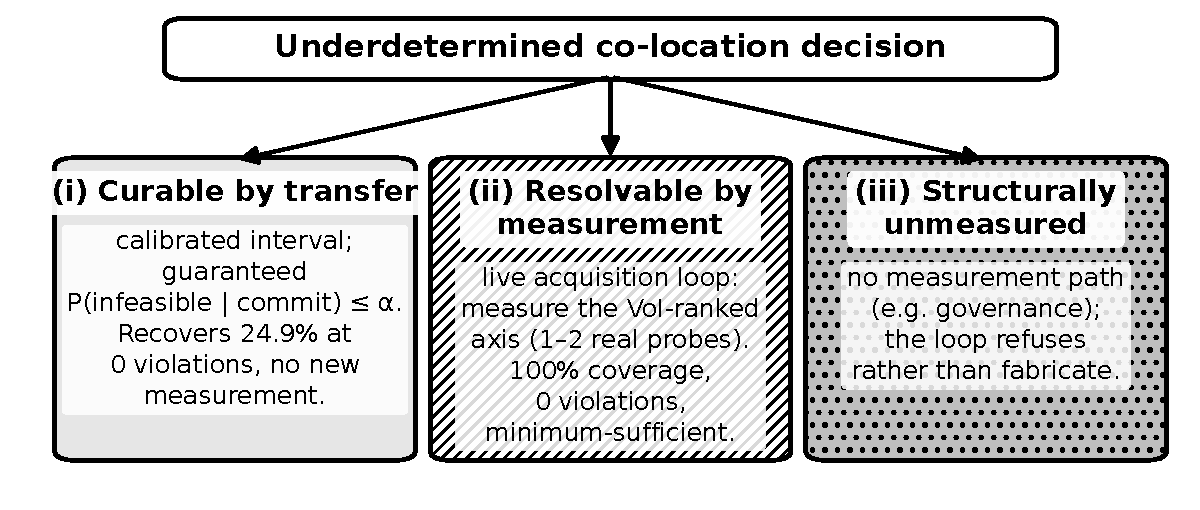
\includegraphics[width=0.86\linewidth]{figures/fig_trichotomy.pdf}
\caption{\textbf{The resolution trichotomy.} Every underdetermined co-location decision is resolved one of three ways: calibrated transfer commits it for free under a feasibility guarantee, the live loop acquires the one measurement that resolves it, or it is structurally unmeasured and the procedure refuses rather than fabricate a value.}
\label{fig:trichotomy}
\end{figure}

\begin{proposition}[Calibrated-transfer feasibility guarantee]
\label{prop:transfer}
Under split-conformal calibration with miscoverage $\alpha$, the commit rule ``commit iff the predicted interval lies entirely on the satisfying side of the threshold'' satisfies $P(\text{committed configuration infeasible}\mid\text{it commits}) \le \alpha$, finite-sample and distribution-free.
\end{proposition}
\emph{Proof sketch.} The split-conformal interval covers the true value with probability $\ge 1-\alpha$ by exchangeability of the calibration and test residuals; a commit fires only when the whole interval satisfies the constraint, so a committed-yet-infeasible event requires the true value to fall outside the interval, of probability $\le\alpha$. \hfill$\square$

\paragraph{Decidability and harm with transfer (30 RouterBench slices, 510 masked-quality decisions).}
Table~\ref{tab:transfer} reports the result through the real verdict. Calibrated transfer recovers \textbf{24.9\%} of decisions made underdetermined by a masked quality cell---committing them rather than abstaining---at \textbf{0} observed hidden violations, against the point imputer's 100\% coverage / \textbf{53.3\%} blind-violation rate and strict selective's 0\% coverage. Recovery is near-constant in $\alpha$ (24.9\%--25.7\%) because the recovered decisions are those where even the widest ($\alpha{=}0.05$) interval is decisive. The split-conformal guarantee holds on the held-out half: interval coverage $0.970/0.927/0.849 \ge 1-\alpha$ and decision-level feasibility error $0.007/0.032/0.046 \le \alpha$ at $\alpha\in\{0.05,0.10,0.20\}$.

\begin{table}[h]
\centering
\caption{\textbf{Calibrated transfer vs.\ baselines on the masked-quality battery} ($n{=}510$). Transfer commits only on a non-straddling calibrated interval; the other ${\sim}75\%$ abstain, certified to require measurement.}
\label{tab:transfer}
\footnotesize
\begin{tabular}{lcc}
\toprule
Rule & Coverage & Hidden-violation rate \\
\midrule
B2 observed-Pareto $=$ B3 median-imputation & 1.00 & 0.533 \\
B5 oracle (sees hidden axis) & 1.00 & 0.000 \\
Strict selective & 0.00 & 0.000 \\
Calibrated transfer ($\alpha{=}0.05$) & \textbf{0.249} & \textbf{0.000} \\
Calibrated transfer ($\alpha{=}0.20$) & 0.257 & 0.000 \\
\bottomrule
\end{tabular}
\end{table}

\emph{Honest scope.} This is \emph{partial} recovery. On the full 30-benchmark cell set the transferable signal is heavy-tailed (the additive predictor's $R^2$ is $0.81$ but a cluster of benchmarks---including MMLU, ARC-challenge, HellaSwag---is near-unpredictable cross-benchmark), so a distribution-free interval tight enough to guarantee $\le5\%$ risk is wide; the $24.9\%$ recovered are decisions where a strong model sits far from the threshold. The $\sim$25\% is a \emph{structural} ceiling, not an artifact of loose intervals: a locally-adaptive (residual-normalized) split-conformal that tightens intervals and commits $32\%$ more held-out cells at $\alpha{=}0.05$---guarantee preserved (coverage $0.952$, feasibility error $0.022$)---leaves decision recovery \emph{unchanged} at $24.9\%$ (Figure~\ref{fig:frontier}), because the limiter is the decision geometry (whether the cheapest contested config's interval resolves), not interval width. The contribution is therefore not ``transfer recovers most decisions''---it is that transfer recovers a \emph{guaranteed} minority safely and \emph{certifies the majority genuinely require measurement}, which is exactly the paper's thesis and the bridge to the loop.

\paragraph{The live acquisition loop, closed with real measurement (full battery).}
The simulated 2.0-vs-6.0 acquisition count (Section~\ref{sec:acq}) is here closed end-to-end (Phase 2 of Algorithm~\ref{alg:resolve}) and swept over the \emph{entire} battery: an underdetermined query triggers the VoI-ranked measurement, whose \emph{measured} value is revealed into the scratch overlay and the verdict re-runs, until commit. Over all \textbf{510} RouterBench decisions (Table~\ref{tab:loop}) the loop commits \emph{every} one with \textbf{0} hidden violations and \textbf{100\%} minimum-sufficient cost. The VoI plan is deterministically optimal---exactly \textbf{1.0} probe when quality is hidden and \textbf{2.0} when quality and cost are both hidden (every one of the 510 decisions, with no exceptions), versus \textbf{2.9}/\textbf{4.0} for random acquisition. Governance has \emph{no} measurement path (Appendix~\ref{app:audit_data}), so when the only remaining blocker is governance the loop \emph{refuses}---raising rather than fabricating a value---and the frozen snapshot is byte-identical after every run. Together with calibrated transfer (which resolves ${\sim}25\%$ for free) this completes a clean three-way split of the co-location gap: curable-by-transfer, resolvable-by-measurement, and structurally-unmeasured.

\begin{table}[h]
\centering
\caption{\textbf{Live acquisition loop over the full RouterBench battery} ($n{=}510$ decisions). Real measurement re-entered through the C7 interface; the frozen snapshot is byte-identical; governance is refused. ``Plan'' is the VoI-ranked acquisition (deterministically the minimal probe count on every decision), ``Rand.'' uniformly-random acquisition.}
\label{tab:loop}
\footnotesize
\setlength{\tabcolsep}{4pt}
\begin{tabular}{lcccccc}
\toprule
Setting & Cov. & Plan probes & Rand.\ probes & Acq.\ cost & Hidden viol. & Min-suff. \\
\midrule
Mask quality (1 blocker) & 1.00 & 1.0 & 2.9 & 0.30 & 0 & 1.00 \\
Mask quality $+$ cost (2 blockers) & 1.00 & 2.0 & 4.0 & 0.35 & 0 & 1.00 \\
\bottomrule
\end{tabular}
\end{table}

\begin{figure}[h]
\centering
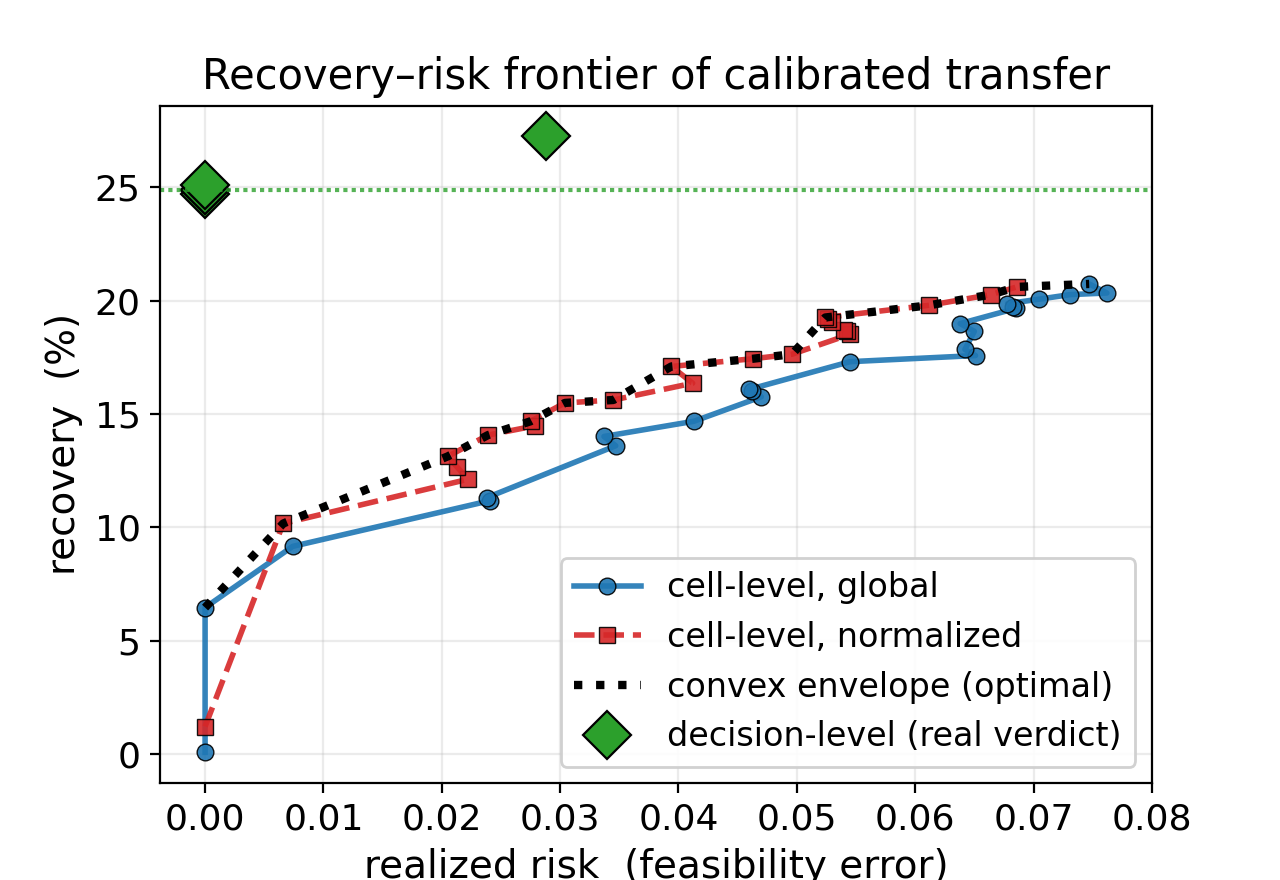
\includegraphics[width=0.62\linewidth]{figures/fig_risk_frontier.png}
\caption{\textbf{The recovery--risk frontier of calibrated transfer.} Sweeping the conformal $\alpha$, cell-level recovery rises with realized risk along a concave frontier; the locally-adaptive (normalized) interval Pareto-dominates the global radius (convex envelope, dashed). But the \emph{decision-level} recovery through the real verdict (green) is capped at ${\sim}25\%$ at zero realized risk---reaching ${\sim}28\%$ only by admitting genuine violations. The ${\sim}25\%$ safe ceiling is structural to the decision geometry, not an artifact of interval width: what transfer cannot recover, the live loop must measure.}
\label{fig:frontier}
\end{figure}

\end{document}
